

\documentclass[11pt,aspectratio=1610]{beamer}	% Available font sizes 8pt, 9pt, 10pt, 11pt, 12pt, 14pt, 17pt, 20pt. Default font size 11pt (corresponds to 22pt at the full screen mode)
\usepackage[utf8]{inputenc}
% 16:10 -> 160x100mm
% 4:3 native slide format 128mm x 96mm

\usetheme{Darmstadt}
\usecolortheme{beaver}
\setbeamercolor{title}{fg=blue}

% \setbeamertemplate{footline}[page number]
% \setbeamertemplate{footline}[frame number]
% \setbeamertemplate{footline}{\hfill\strut\insertframenumber\quad\quad}
% \setbeamertemplate{footline}{\hfill\strut\footnotesize\insertpagenumber\quad\quad}
\setbeamertemplate{navigation symbols}{\insertslidenavigationsymbol\insertbackfindforwardnavigationsymbol\quad\hfill\strut\footnotesize\insertframenumber\quad}

\usepackage{natbib}	%defines citation style
% \citestyle{aa}

\usepackage{caption}
\captionsetup[figure]{labelformat=empty,singlelinecheck=false,aboveskip=1pt,justification=raggedright,font=scriptsize}
\newcommand{\captionoftiny}[2]{\captionof{#1}{\color{gray} \tiny #2}}

\setbeamercolor{button}{bg=white,fg=gray}

\usepackage{siunitx}
	\DeclareSIUnit[number-unit-product=\,]\au{au}
	\DeclareSIUnit[number-unit-product=\,]\nT{\nano\tesla}
	\DeclareSIUnit[number-unit-product=\,]\Rs{\textit{R}_\sun{}}
	\DeclareSIUnit[number-unit-product=\,]\RE{\textit{R}_E}
	\sisetup{table-figures-uncertainty=2, table-number-alignment=center, range-phrase=--, range-units=single}

\mode<handout>{
	\usepackage{pgfpages}
	\pgfpagesuselayout{16 on 1}[a4paper,border shrink=8mm,landscape]

	\setbeamercolor{background canvas}{bg=black!2}
}


% maltes_commands.tex
% full journal name replacement
\def\aj{{Astron.~J.}}				%\def\aj{{AJ}}
\def\araa{{Ann.~Rev.~Astron.~Astrophys.}}	%\def\araa{{ARA\&A}}
\def\apj{{Astrophys.~J.}}			%\def\apj{{ApJ}}
\def\apjl{{Astrophys.~J.,~Lett.}}		%\def\apjl{{ApJ}}
\def\mnras{{Mon.~Not.~R.~Astron.~Soc.}}		%\def\mnras{{MNRAS}}
\def\aap{{Astron.~Astrophys.}}			%\def\aap{{A\&A}}
\def\nat{{Nature}}				%\def\nat{{Nat}}
\def\apjs{{Astrophys.~J.,~Suppl.~Ser.}}		%\def\apjs{{ApJS}}
\def\pasp{{Publ.~Astron.~Soc.~Pac.}}		%\def\pasp{{PASP}}

% other short commands
\def\ion#1#2{{\rm #1}{\sc #2}}
\newcommand{\Hi}{\ion{H}{i}}
\newcommand{\Hii}{\ion{H}{ii}}

% new since 2015
\def\planss{{Planet.~Space~Sci.}}		%Planetary and Space Science
\def\grl{{Geophys.~Res.~Lett.}}			%Geophysical Research Letters
\def\ssr{{Space~Sci.~Rev.}}			%Space Science Reviews
\def\jgr{{J.~Geophys.~Res.}}			%Journal of Geophysical Research

% new since 2016-10-20
\newcommand{\Rsun}{$R_\odot$}
\def\solphys{{Solar~Phys.}}			%\def\solphys{{SoPh}}	%Solar Physics
\def\aapr{{Astron.~Astrophys.~Rev.}}		%\def\aapr{{A\&ARv}}	%The Astronomy and Astrophysics Review

% new since 2017-10-05
\newcommand{\Kp}{\textit{Kp}}

% new since 2017-11-04
\def\zap{{Z.~Astrophys.}}			%\def\zap{{ZAp}}	%Zeitschrift für Astrophysik
\def\procspie{{Proc.~SPIE}}			%Proceedings of the SPIE

% new since 2017-11-16
\def\qjras{{Quart.~J.~R.~Astron.~Soc.}}		%\def\qjras{{QJRAS}}	%Quarterly Journal of the Royal Astronomical Society

% new since 2018-01-28
\newcommand*{\sun}{\ensuremath{\odot}}
\newcommand{\Rs}{$R_\sun{}$}

\newcommand{\vBz}{$vB_\text{z}$}

% new since 2018-04-07
\newcommand{\RE}{$R_\text{E}$}		%\Re already exists...

% new since 2018-06-16
\def\rsquo{{'}}
\def\aaps{{Astron.~Astrophys.,~Suppl.~Ser.}}	%\def\aap{{A\&AS}}	%Astronomy and Astrophysics Supplement Series

% new since 2018-07-29
% get abbreviations from NLM catalog: https://www.ncbi.nlm.nih.gov/nlmcatalog
% search and replace the following abbreviations
% \def\jgra{{J.~Geophys.~Res.~Space~Phys.}}	%Journal of Geophysical Research (Space Physics)
% \def\lrsp{{Living~Rev.~Sol.~Phys.}}		%Living Reviews in Solar Physics
% \def\jswsc{{J.~Space~Weather~Space~Clim.}}	%Journal of Space Weather and Space Climate



% title slide
\title[Solar wind]{The solar wind's geomagnetic impact and its Sun–Earth evolution}
\subtitle{Predictive models for space weather and for the Parker Solar Probe orbit}
\author[MV]{PhD defense by\\\textit{Malte Venzmer}}
\institute[IAG]{
	\begin{columns}[c]
	\column{0.1\textwidth}
	\column{0.4\textwidth}

		PhD student\\
		within the doctoral program ProPhys,\\
		Georg-August University School of Science (GAUSS)\\
		\ \\
		Institute for Astrophysics\\
		Georg-August Universität Göttingen

	\column{0.1\textwidth}
	\column{0.4\textwidth}

		\underline{Examination board members}\\
		Dr. Volker Bothmer (supervisor, referee)\\
		Prof. Dr. Ansgar Reiners (2nd referee)\\
		Prof. Dr. Stefan Dreizler\\
		Prof. Dr. Wolfram Kollatschny\\
		Prof. Dr. Hardi Peter\\
		Prof. Dr. Andreas Tilgner
	\end{columns}
}
% \date{\today}
\date[2018]{\vspace*{0.5cm}\\ Thursday, 1 November 2018, 14:00\\Seminarraum Astrophysik (SR 17, F 05.104)}
\subject{Solar wind}
% \logo{
\includegraphics[height=1cm]{figures/IAG_LogoRGB.png}}


\begin{document}

\AtBeginSection[]{
	\subsection{}	% for making the nav dots appear
	\frame{\tableofcontents[currentsection]}
}

\frame[plain]{\titlepage}

\begin{frame}[c]{Two topics}{}
	\onslide*<1>{
	\begin{block}{Title}
		\centering{
		The solar wind's geomagnetic impact and its Sun–Earth evolution\\
		--\\
		Predictive models for space weather and for the Parker Solar Probe orbit
		}\\
	\end{block}
	}
	
	\begin{block}<2->{Study 1}
		The solar wind's geomagnetic impact -- Predictive models for space weather
	\end{block}
	\begin{block}<3>{Study 2}
		The solar wind's Sun–Earth evolution -- Predictive models for the Parker Solar Probe orbit
	\end{block}
\end{frame}


\section{Solar wind}

\begin{frame}[c]{Solar wind}{}
	\begin{columns}[c]
	\column{0.5\textwidth}

	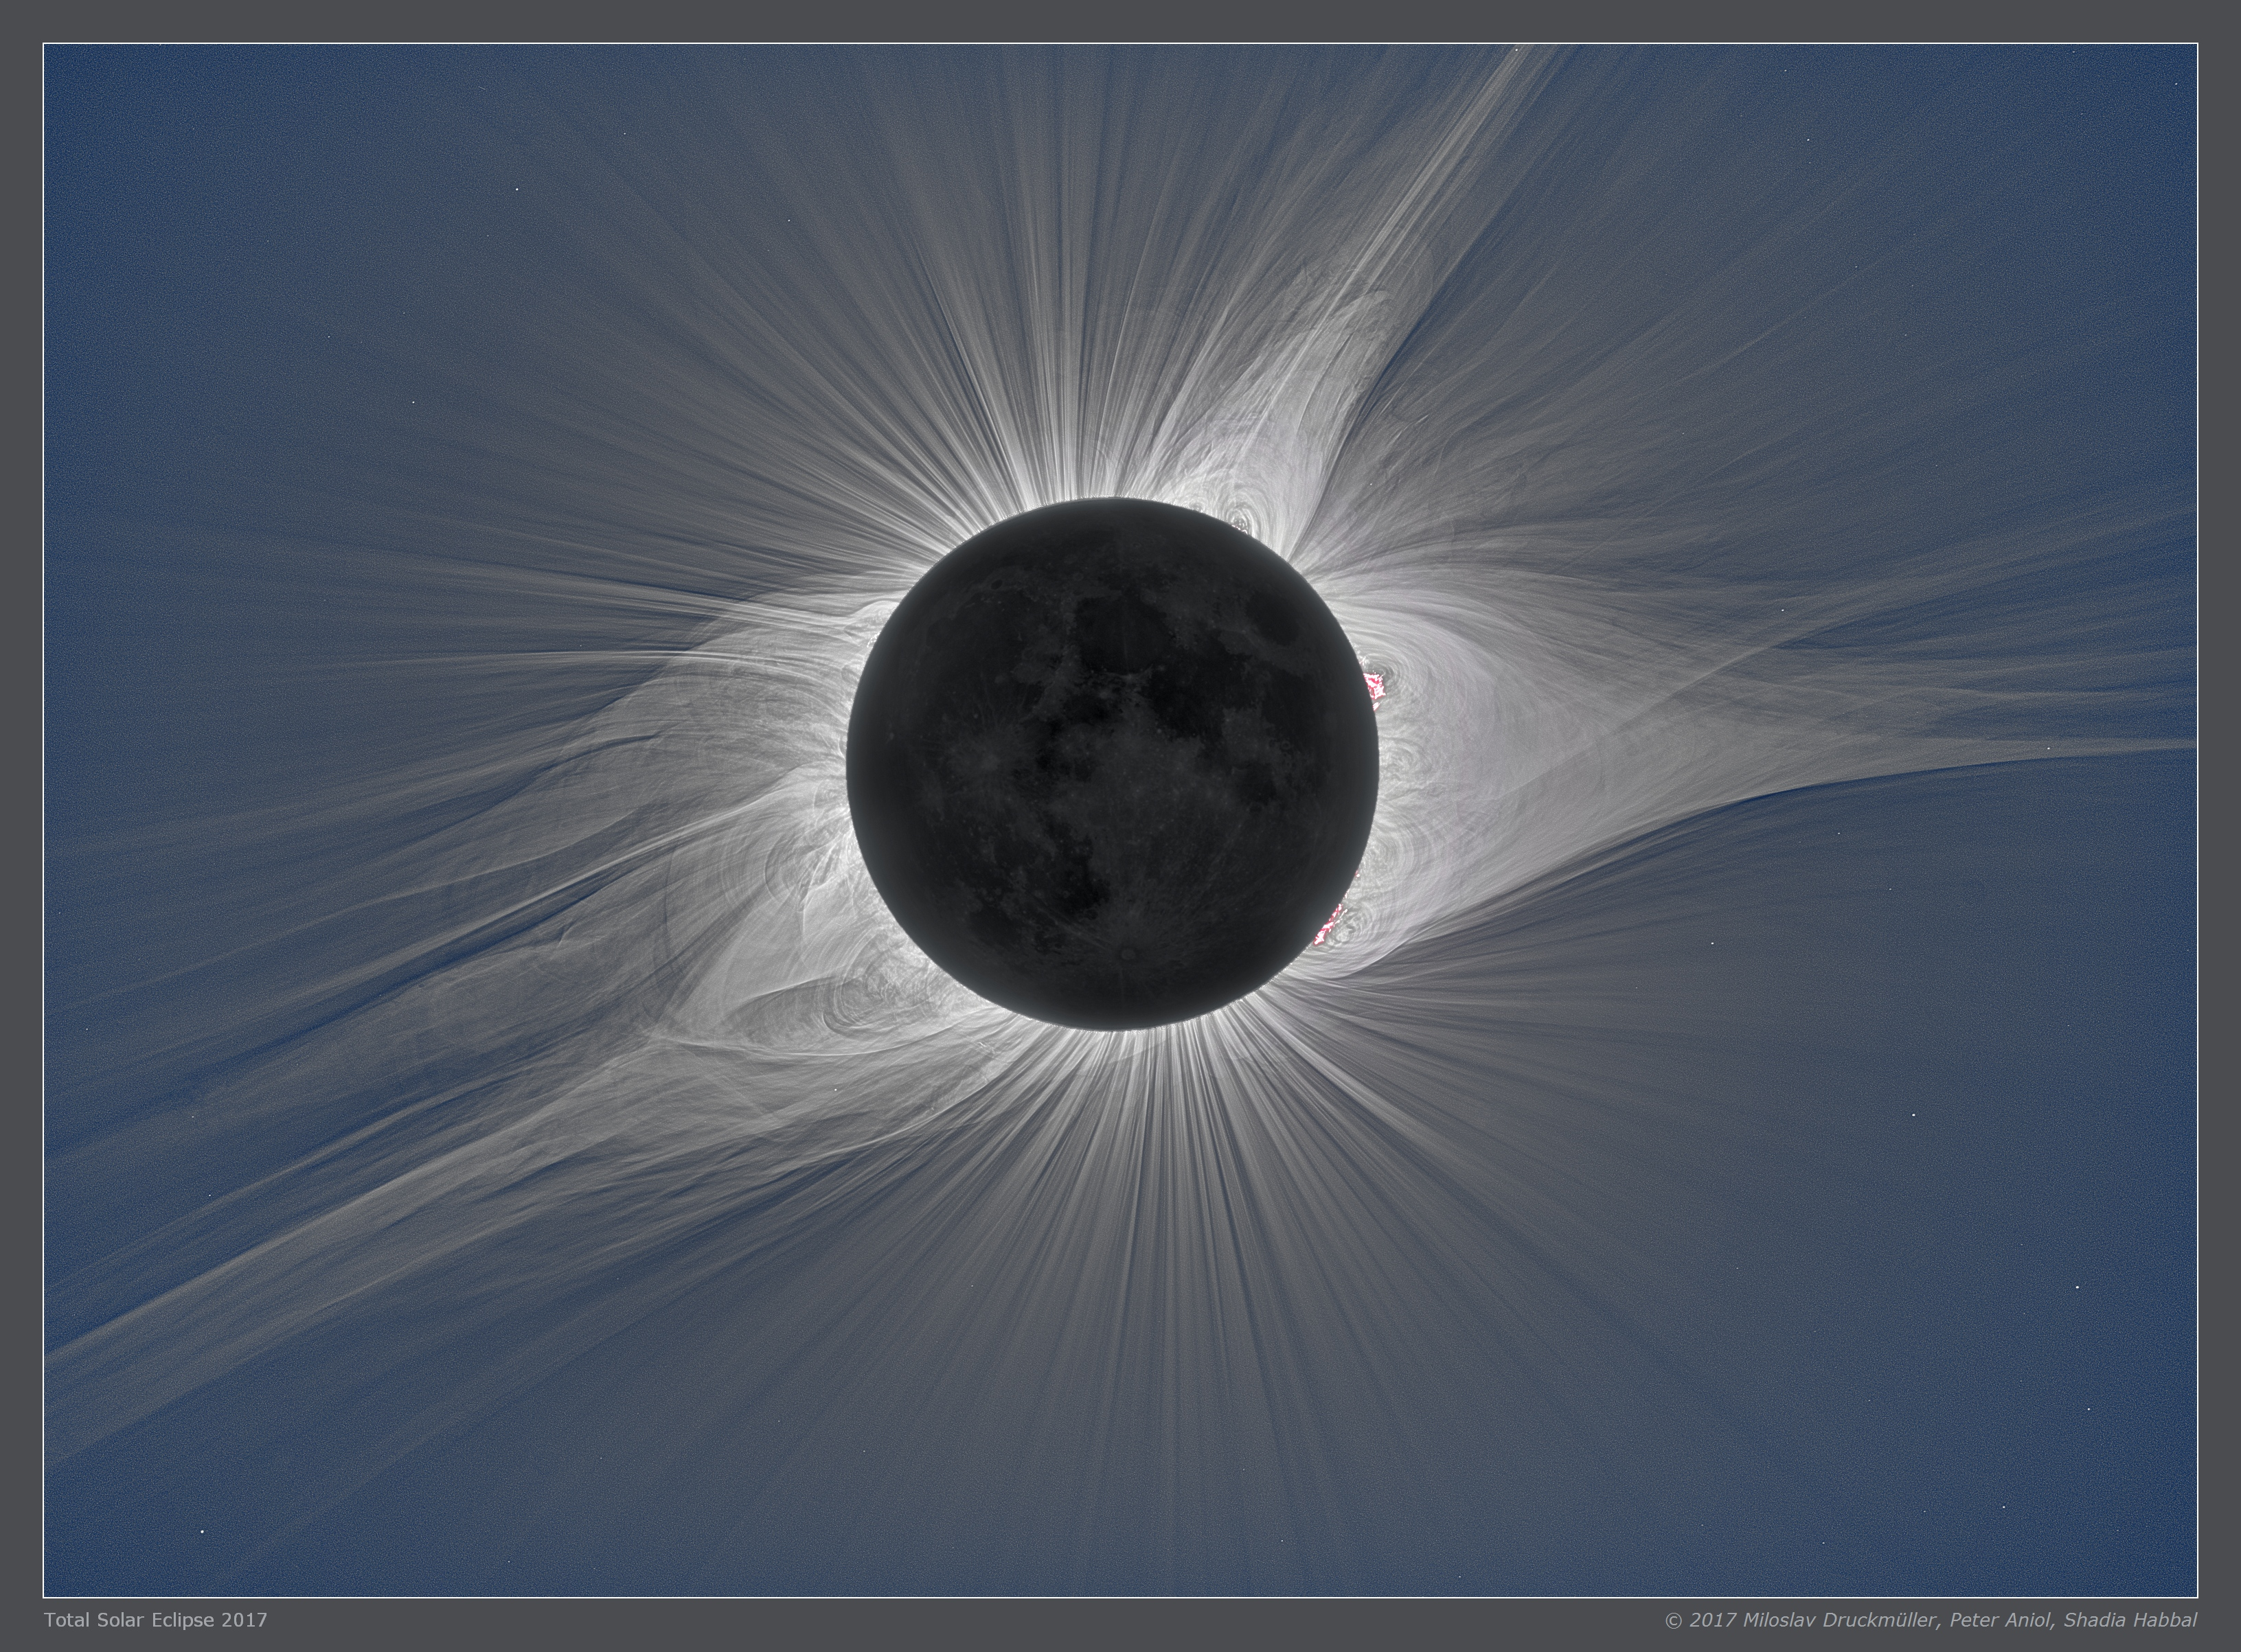
\includegraphics[width=\textwidth]{../figures_of_others/images/Tse_2017_mi800.jpg}
	\captionoftiny{figure}{\centering Credit: \href{http://www.zam.fme.vutbr.cz/~druck/Eclipse/}{Miloslav Druckmüller, Peter Aniol, Shaddia Habbal}, 2017}
	
	\column{0.5\textwidth}
	
	- flow of magnetized plasma\\
	- consists of electrons, protons and 5\% helium
	
	\end{columns}
\end{frame}
\begin{frame}[c]{Solar wind}{}
	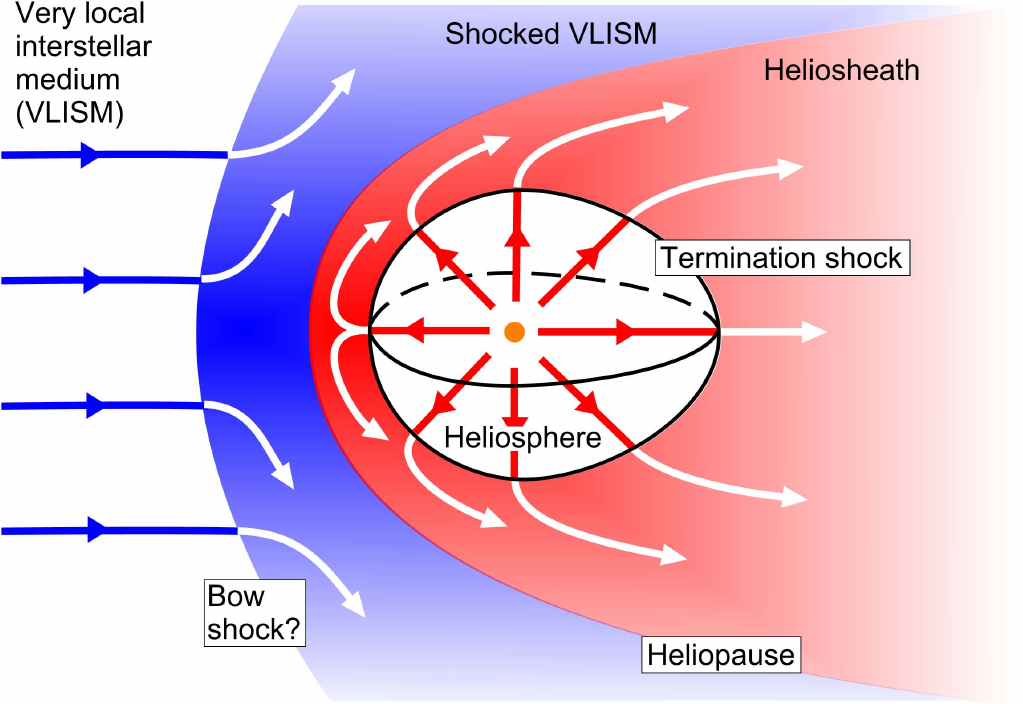
\includegraphics[width=0.7\textwidth]{../figures_of_others/images/Owens2013_Heliosphere_screenshot.png}
	\captionoftiny{figure}{Credit: {\citet[Fig.~9]{Owens2013}}}
\end{frame}
\begin{frame}[c]{Solar wind}{}
	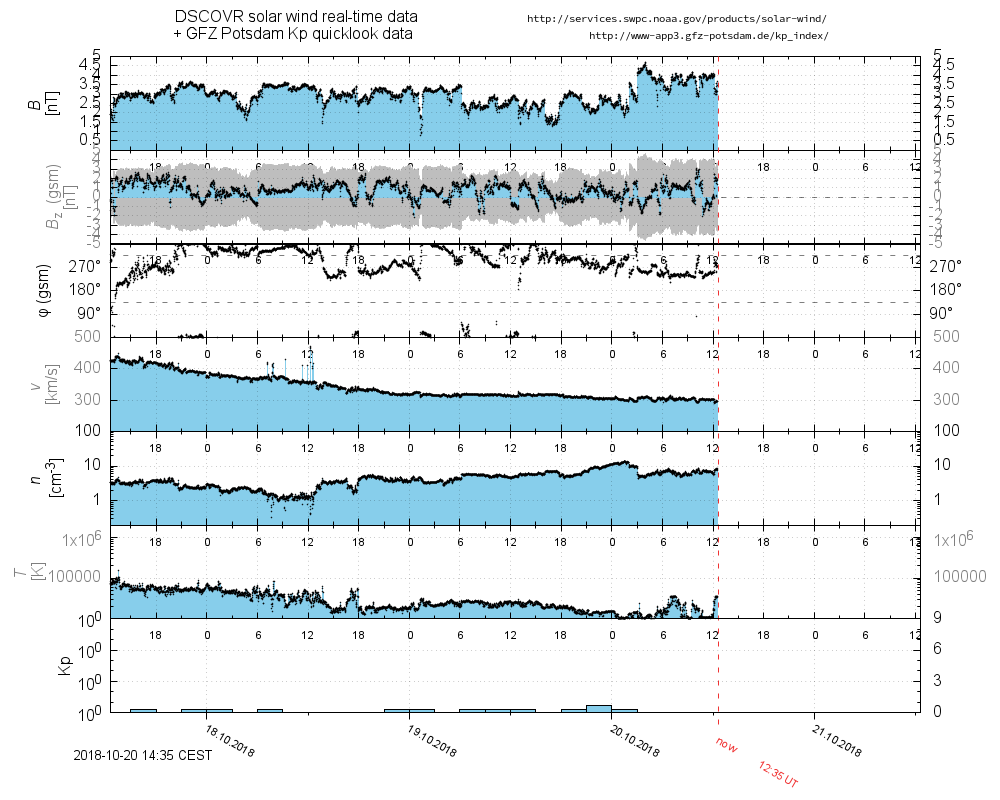
\includegraphics[width=0.7\textwidth]{../talk_figures/ace_realtime_ap_plot.png}
% 	\captionoftiny{figure}{}
\end{frame}

\begin{frame}[c]{Solar magnetic field}{}
	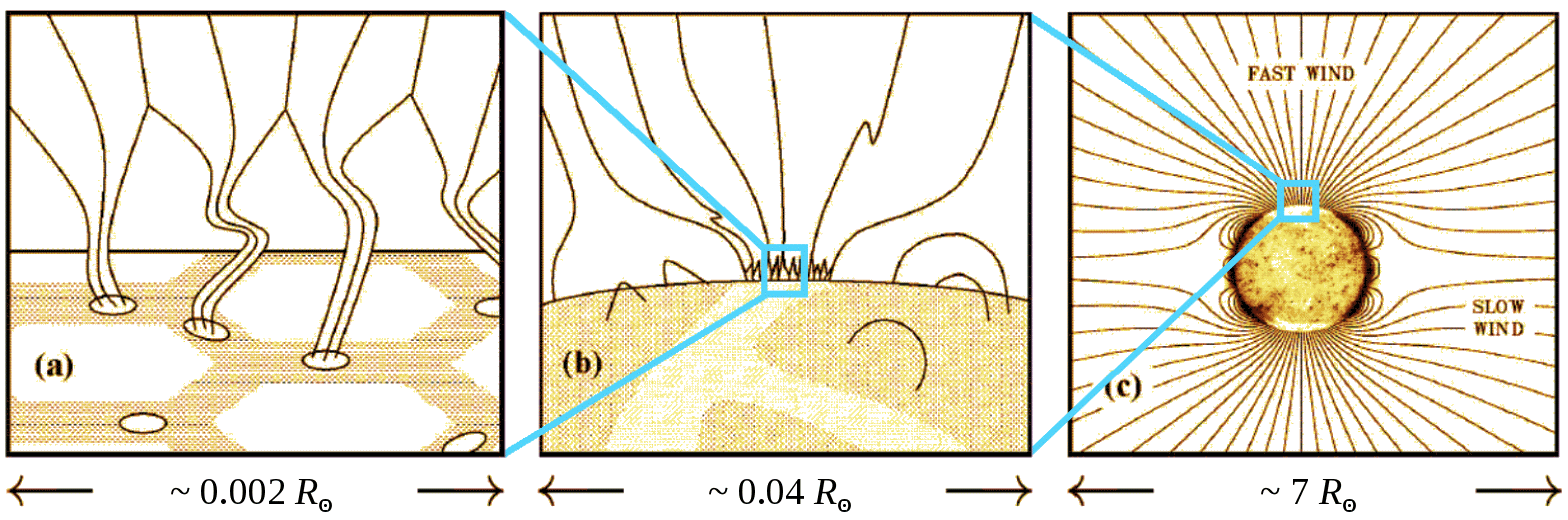
\includegraphics[width=0.8\textwidth]{../figures_of_others/images/Cranmer2005_fig1_color.png}
	\captionoftiny{figure}{Courtesy of S. R. Cranmer}
\end{frame}
\begin{frame}[c]{Solar magnetic field}{}
	\begin{columns}[c]
	\column{0.5\textwidth}

	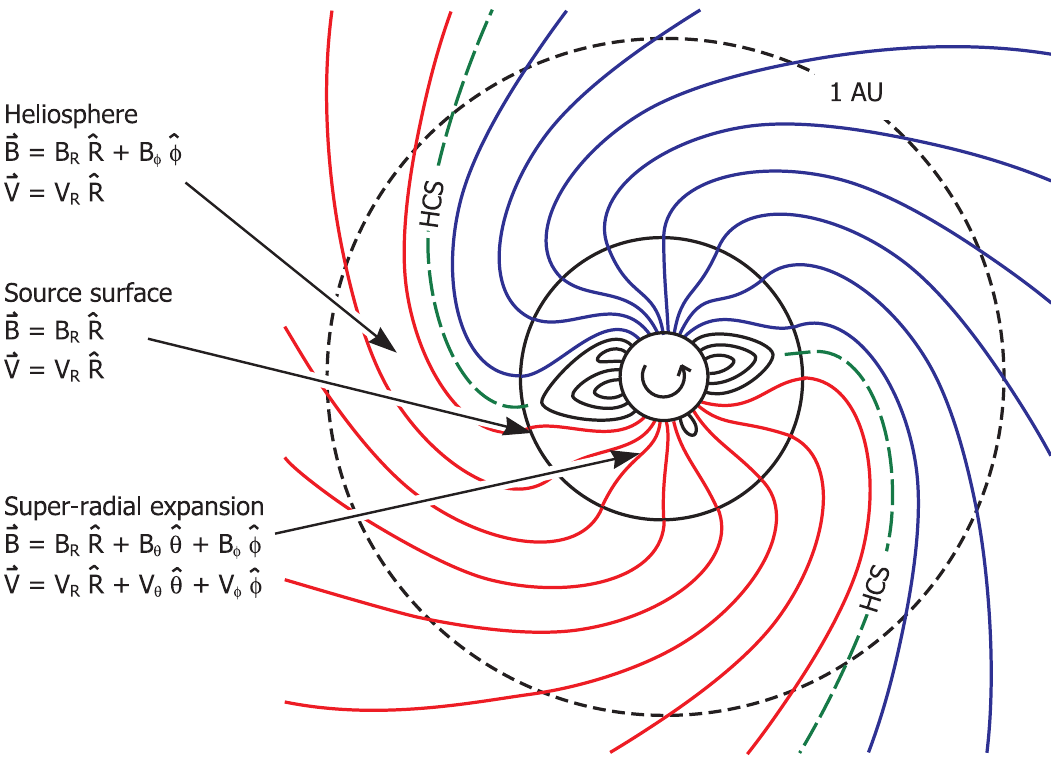
\includegraphics[width=\textwidth]{../figures_of_others/images/Owens2013_PFSS_Sectors_screenshot.png}
	\captionoftiny{figure}{Credit: {\citet[Fig.~1]{Owens2013}}, adapted from {\citet[Fig.~1]{Schatten1969}}}
	
	\column{0.5\textwidth}
	
	\end{columns}
\end{frame}
\begin{frame}[c]{Slow and fast solar wind}{}
	\begin{columns}[c]
	\column{0.5\textwidth}

	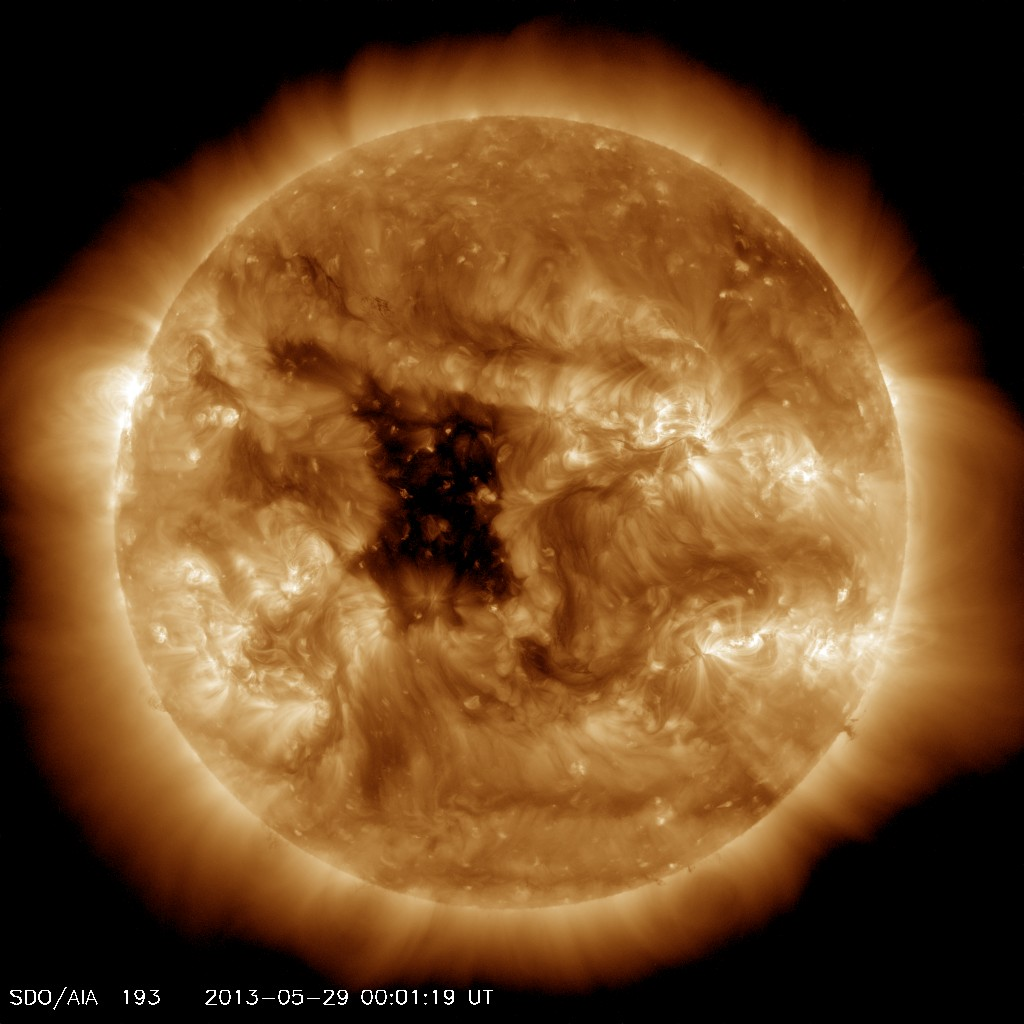
\includegraphics[width=\textwidth]{../figures_of_others/images/20130529_000119_1024_0193.jpg}
	\captionoftiny{figure}{Credit: NASA/SDO and the AIA, EVE and HMI science teams}
	
	\column{0.5\textwidth}
	
	\end{columns}
\end{frame}
\begin{frame}[c]{Slow and fast solar wind}{}
	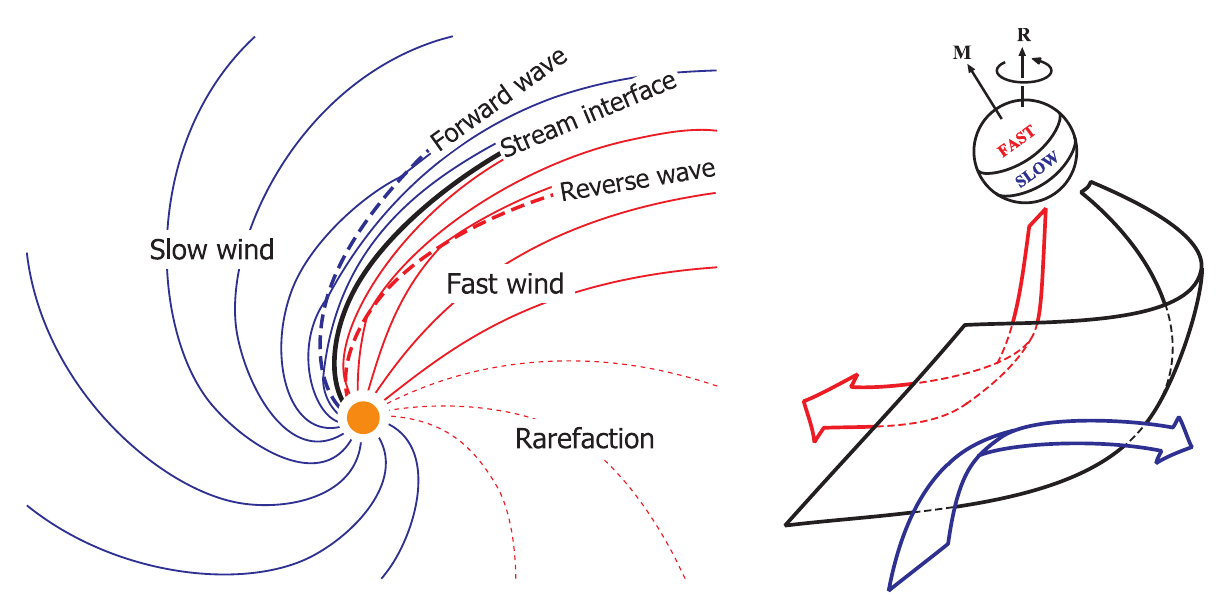
\includegraphics[width=0.8\textwidth]{../figures_of_others/images/Owens2013_CIR_2panel_screenshot.png}
	\captionoftiny{figure}{Credit: {\citet[Fig.~7]{Owens2013}}; right panel adapted from {\citet[Fig.~2]{Pizzo1991}}}
\end{frame}
\begin{frame}[c]{Solar wind}{In-situ example}
	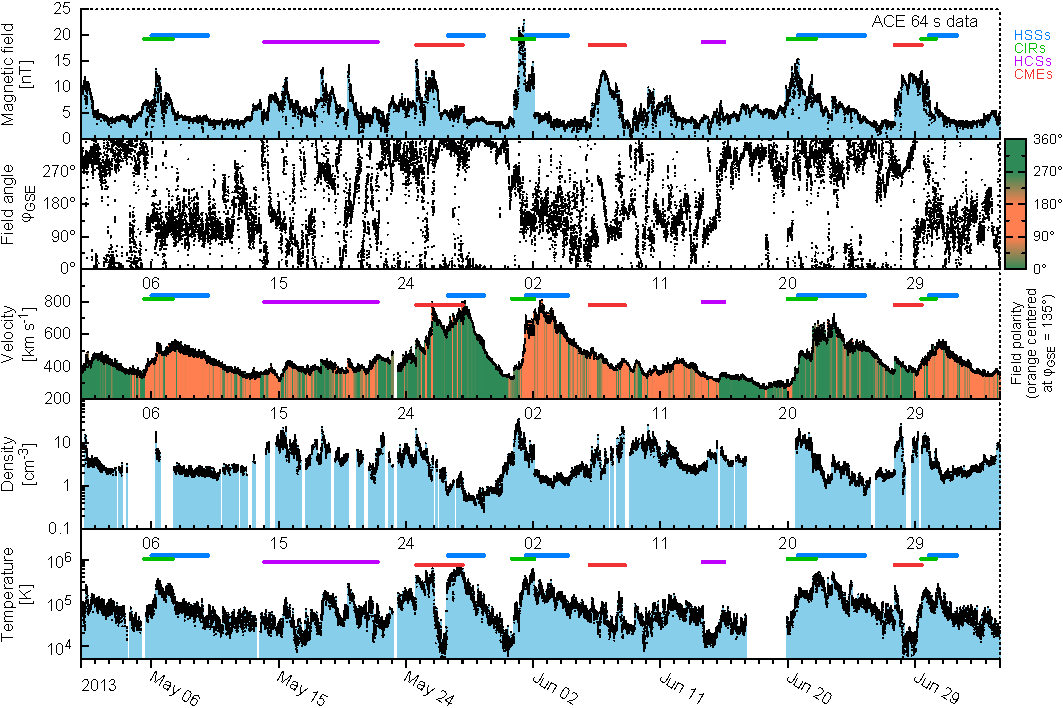
\includegraphics[width=0.8\textwidth]{../figures_of_mine/gnuplots/ACE_64s_v7_thesis_CIRs_2013-5-1_65_plot.pdf}
% 	\captionoftiny{figure}{}
\end{frame}

\begin{frame}[c]{Solar activity}{Sunspots}
	\centering
% 	\includegraphics[width=0.7\textwidth]{../figures_of_others/images/}
	\captionoftiny{figure}{}
\end{frame}
\begin{frame}[c]{Solar activity}{}
	\centering
	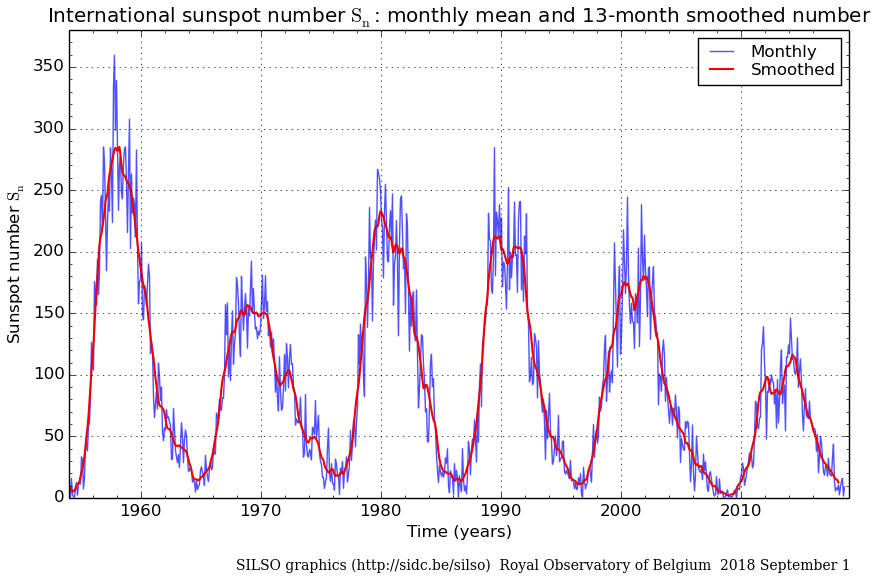
\includegraphics[width=0.7\textwidth]{../figures_of_others/images/ROB_SILSO_SSN_wolfmms_cropped.png}
% 	\captionoftiny{figure}{Credit: \href{http://sidc.be/silso/monthlyssnplot}{SILSO data/image, Royal Observatory of Belgium, Brussels}, 2018}

	\vfill\hfill \hyperlink{butterfly}{\beamerskipbutton{Magnetic butterfly diagram}}
\end{frame}
\begin{frame}[c]{Solar activity}{}
	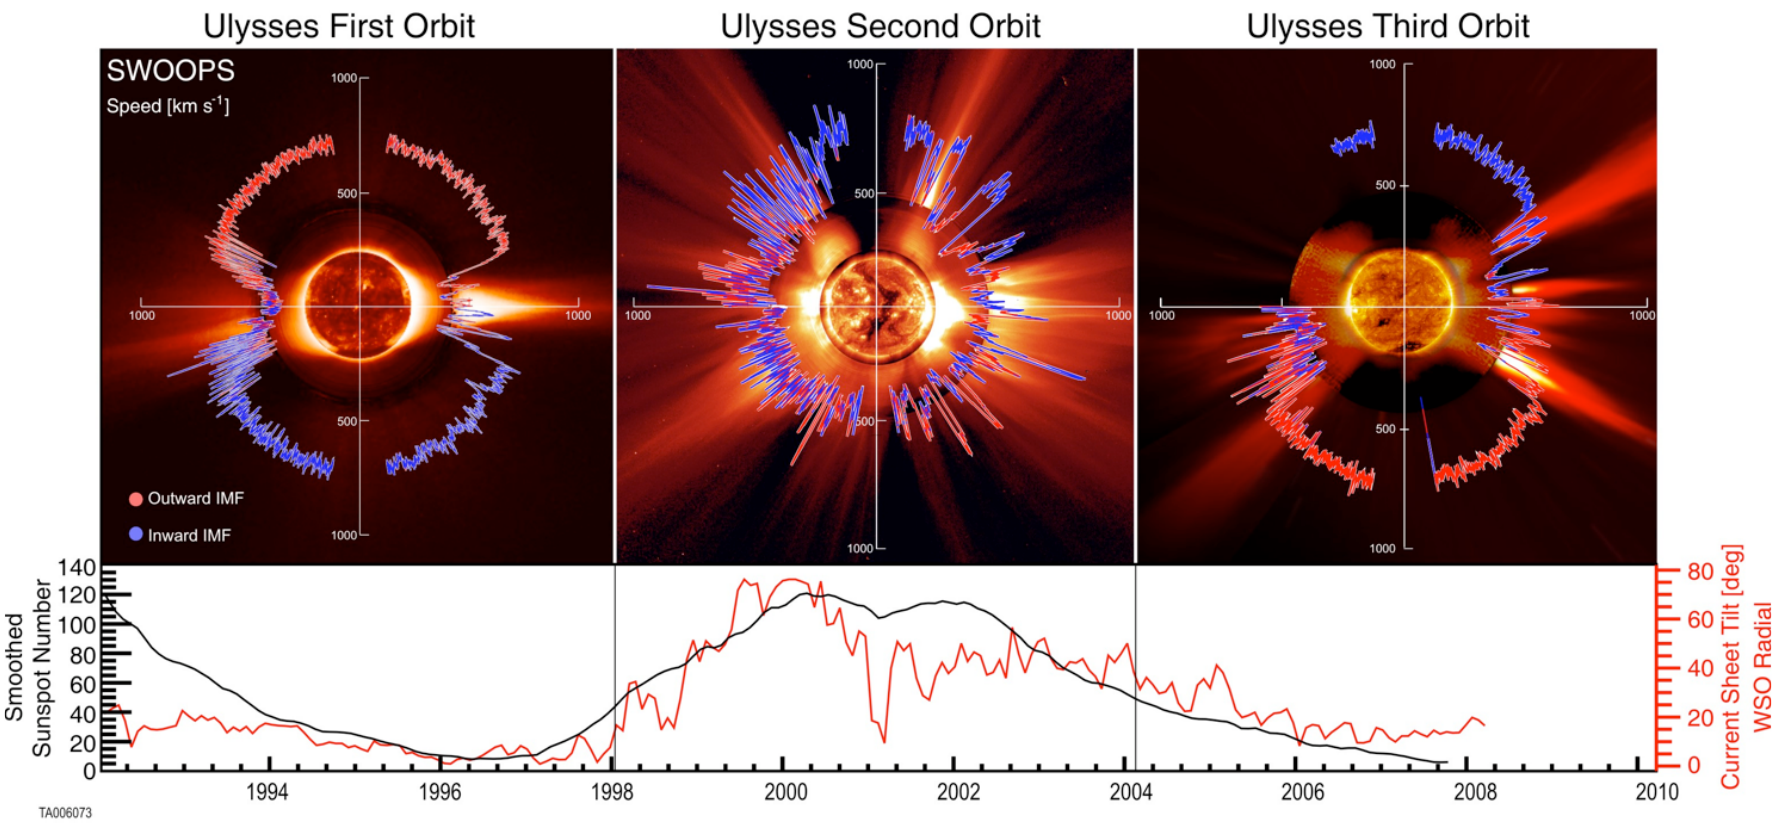
\includegraphics[width=0.9\textwidth]{../figures_of_others/images/McComas2008_Ulysses_orbit_.png}
	\captionoftiny{figure}{Credit: {\citet[Fig.~1]{McComas200809}}}
\end{frame}

\begin{frame}[c]{Coronal mass ejections}{}
	\begin{columns}[c]
	\column{0.5\textwidth}
	
		\onslide*<1-2>{
		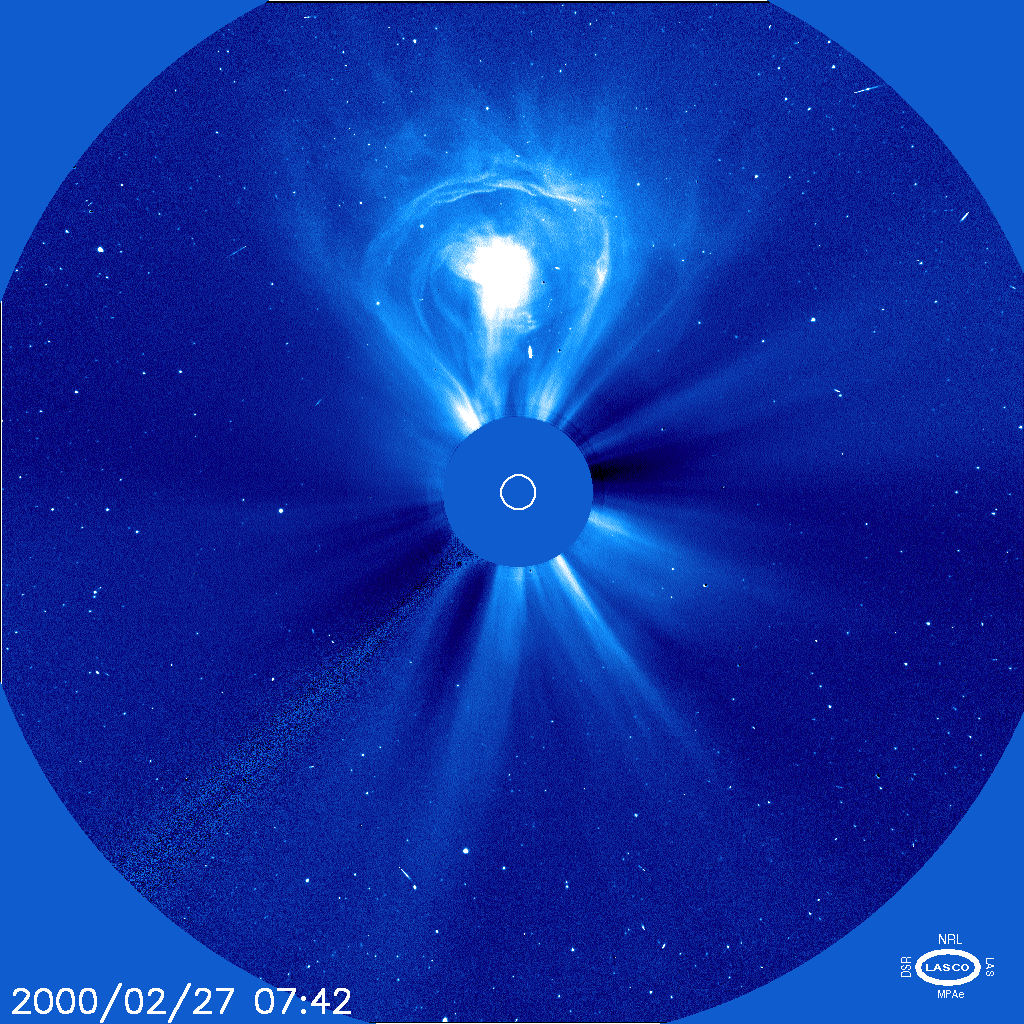
\includegraphics[height=\textwidth]{../figures_of_others/images/20000226_lightbulb_CME_c3full.png}
		\captionoftiny{figure}{Courtesy of SOHO/LASCO consortium. SOHO is a project of international cooperation between ESA and NASA}
		}
		\onslide*<3>{
		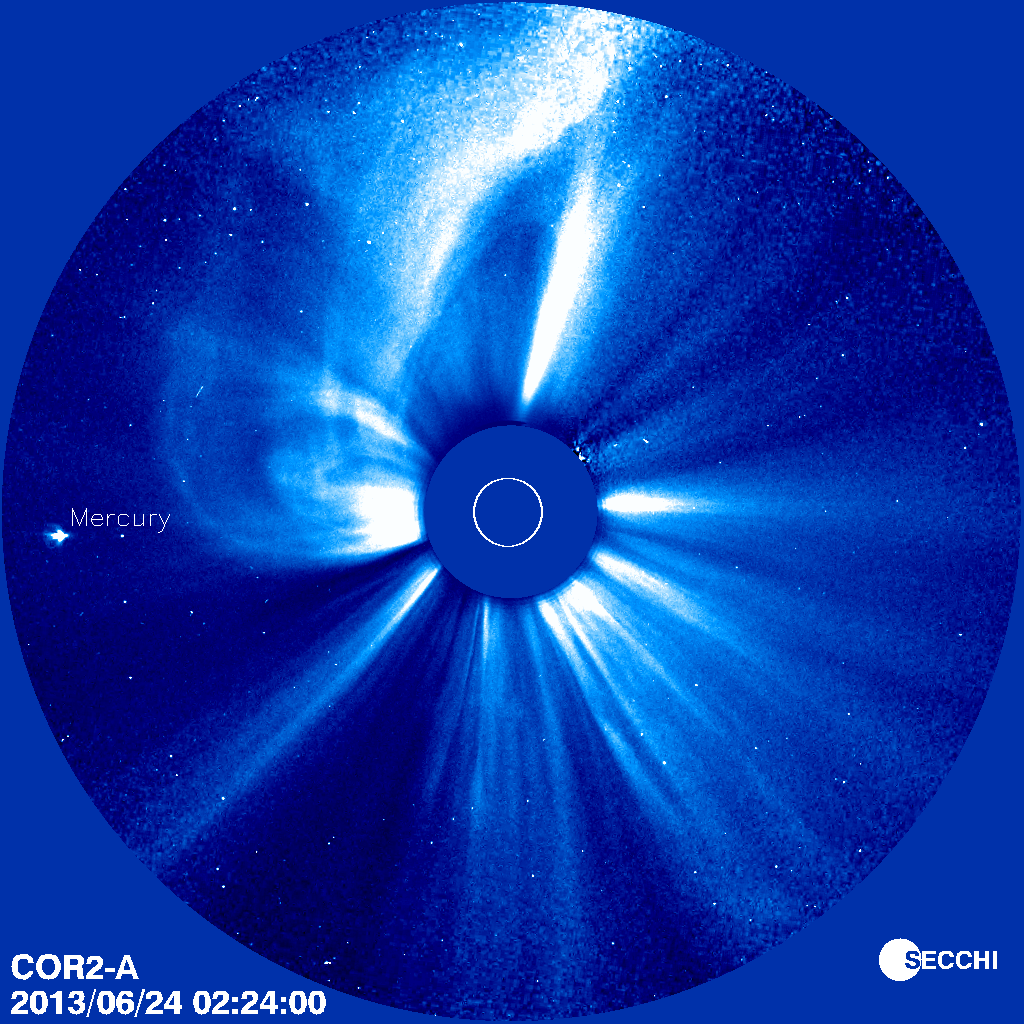
\includegraphics[height=\textwidth]{../figures_of_others/images/STEREO_A_COR2_20130624_022400_dbc2A.png}
		\captionoftiny{figure}{Courtesy of \href{https://stereo.gsfc.nasa.gov/gallery/copyright.shtml}{STEREO/COR2 consortium (NASA)}\\\ }
		}
		
		\onslide*<4>{
		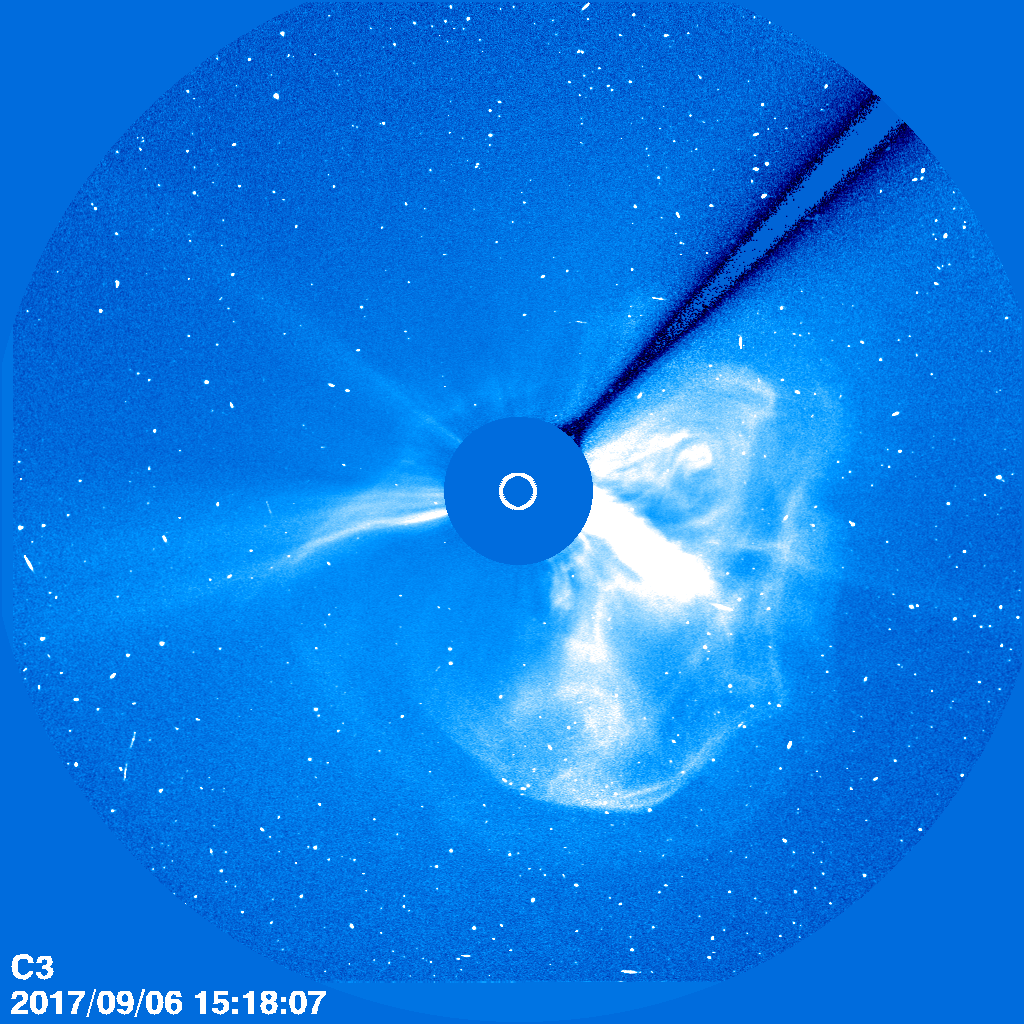
\includegraphics[height=\textwidth]{../figures_of_others/images/SOHO_LASCO_C3_20170906_151807.png}
		\captionoftiny{figure}{Courtesy of SOHO/LASCO consortium; SOHO is a project of international cooperation between ESA and NASA}
		}
	
	\column{0.05\textwidth}
	
	\column<2->{0.45\textwidth}

		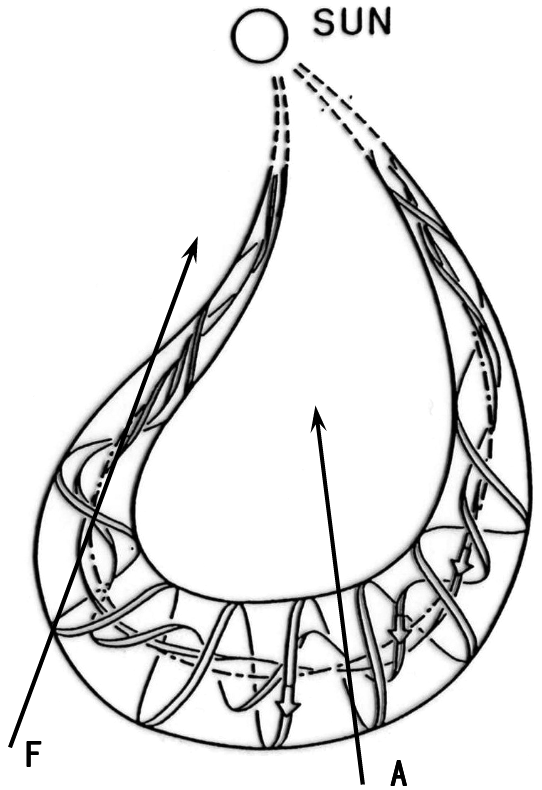
\includegraphics[height=0.9\textwidth]{../figures_of_others/images/Marubashi2007_fig1.png}
		\captionoftiny{figure}{Credit: {\citet[Fig.~1, panel (a)]{Marubashi2007}}\\\ }
		
	\end{columns}
\end{frame}
\begin{frame}[c]{CME orientation}{}
	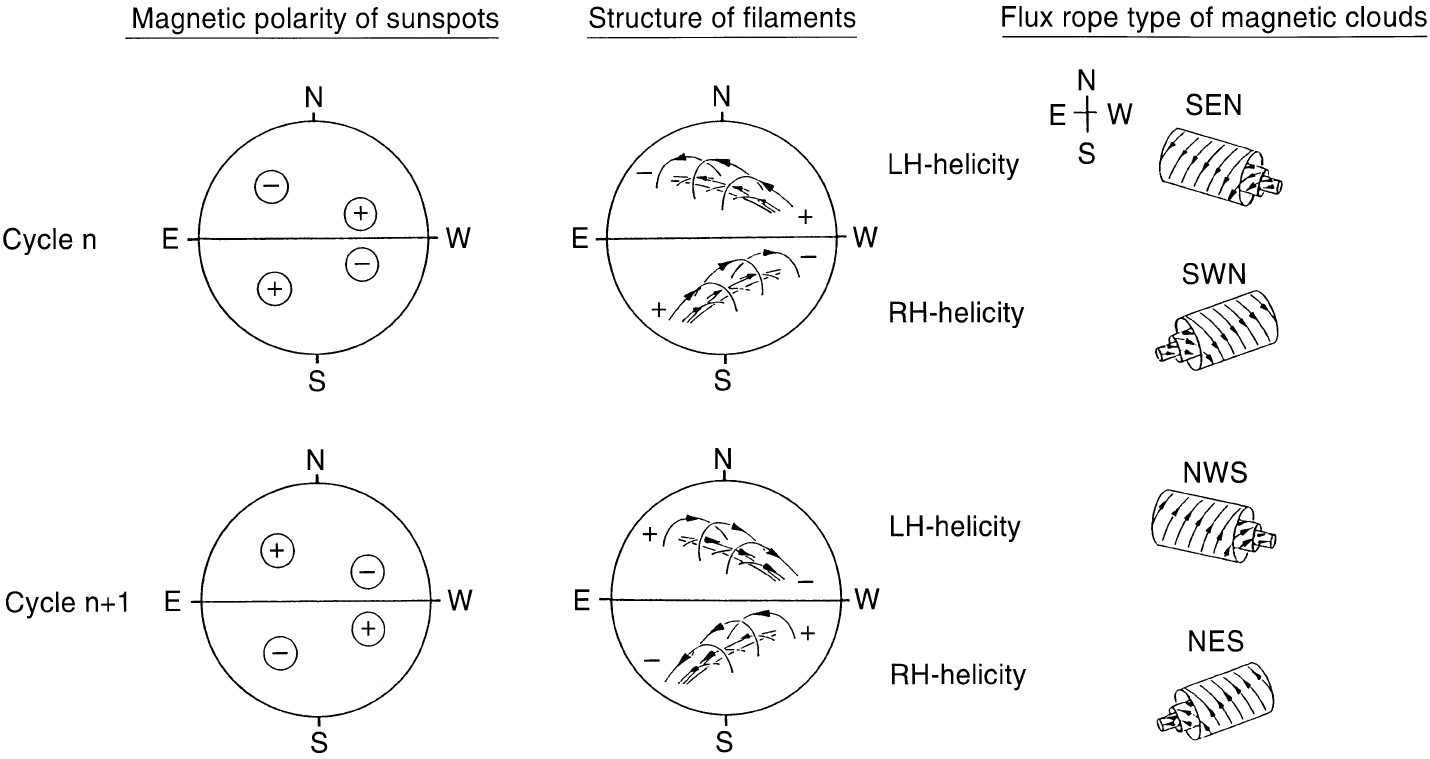
\includegraphics[width=0.7\textwidth]{../figures_of_others/images/Bothmer1998_fig18.png}
	\captionoftiny{figure}{Credit: {\citet[Fig.~18]{Bothmer1998}}}
\end{frame}
\begin{frame}[c]{In-situ CMEs}{}
	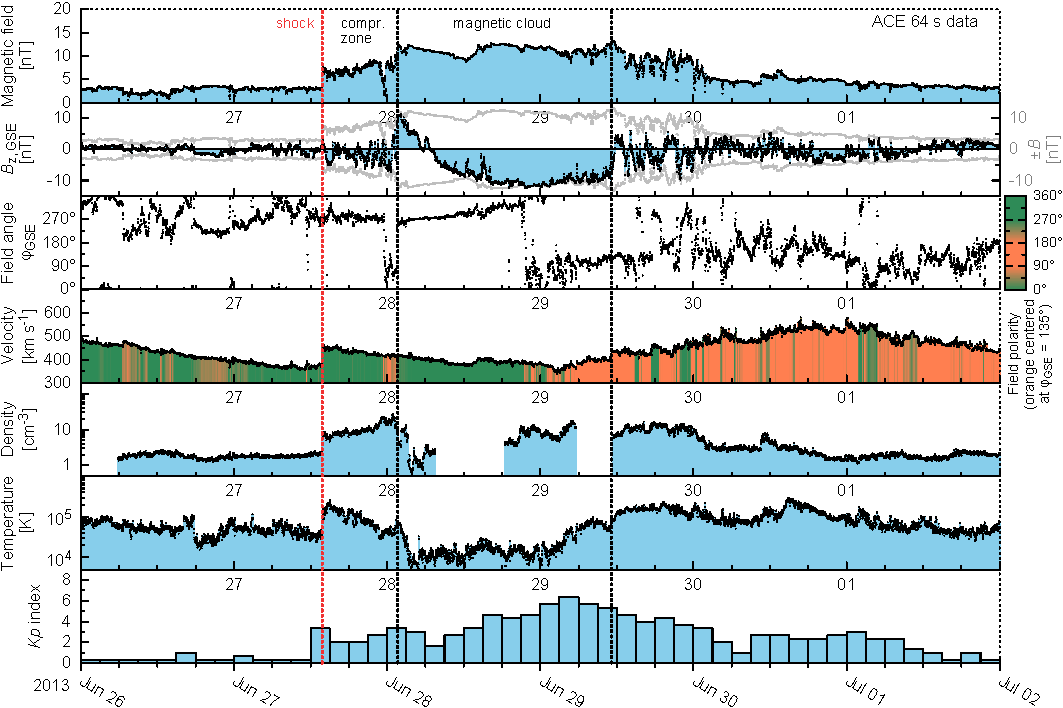
\includegraphics[width=0.8\textwidth]{../figures_of_mine/gnuplots/ACE_64s_v7_thesis_CME_2013-6-26_6.pdf}
% 	\captionoftiny{figure}{}
\end{frame}
\begin{frame}[c]{Solar wind and CME forecast}{}
	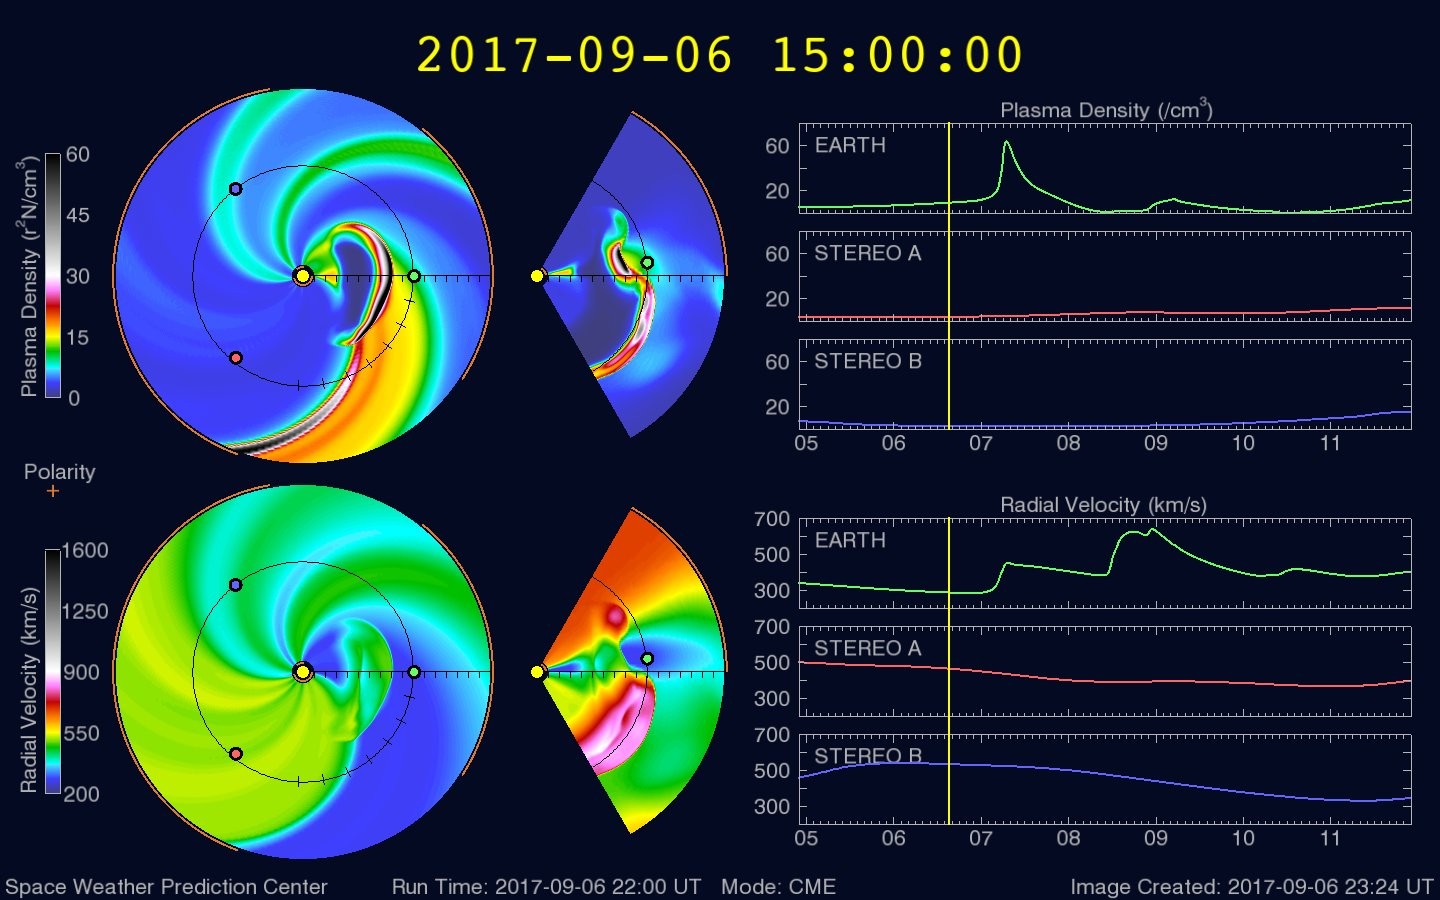
\includegraphics[width=0.8\textwidth]{../figures_of_others/images/enlil_com1_20170906T150000.jpg}
	\captionoftiny{figure}{Credit: \href{http://dx.doi.org/10.7289/V5445JGH}{SWPC: WSA-Enlil Solar Wind Prediction. NOAA National Centers for Environmental Information}}
\end{frame}


\section{Geomagnetic impact of the solar wind}

\begin{frame}[c]{Geomagnetic impact of the solar wind}{}
	images...
\end{frame}
\begin{frame}[c]{Geomagnetic impact of the solar wind}{Aims}
	Empirical relations to predict the \Kp~index from solar wind electric field and from CME and stream velocity
\end{frame}

\begin{frame}[c]{Magnetosphere}{}
	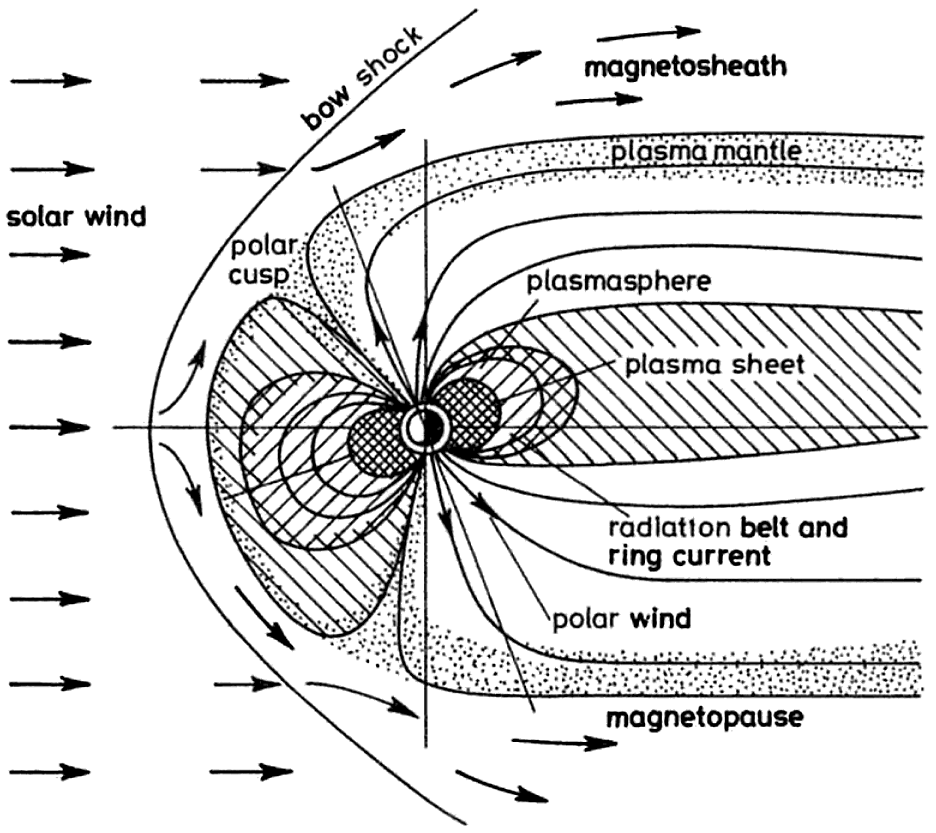
\includegraphics[width=0.5\textwidth]{../figures_of_others/images/Davies1990_magnetosphere_sharpened.png}
	\captionoftiny{figure}{Credit: {\citet[Fig.~2.12]{Davies1990}}}
\end{frame}
\begin{frame}[c]{Magnetosphere}{}
	4 interaction mechanisms
\end{frame}
\begin{frame}[c]{Magnetosphere}{}
	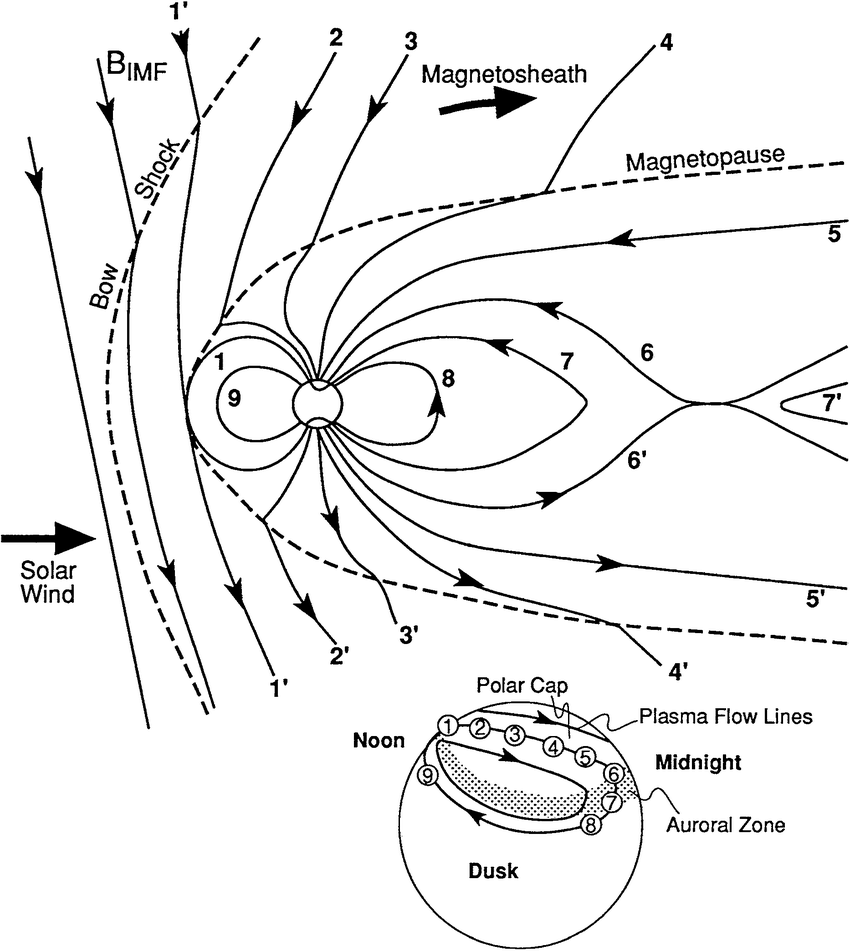
\includegraphics[width=0.5\textwidth]{../figures_of_others/images/Kivelson1995_fig9_11_dungey_cycle.png}
	\captionoftiny{figure}{Credit: {\citet[Fig.~9.11]{Hughes1995}}}
\end{frame}
\begin{frame}[c]{Magnetosphere}{}
	4 factors for merging flux rate
\end{frame}

\begin{frame}[c]{\Kp~index}{}
	\begin{columns}[c]
	\column{0.5\textwidth}
		
		13 observatories...
		
	\column{0.5\textwidth}
		
		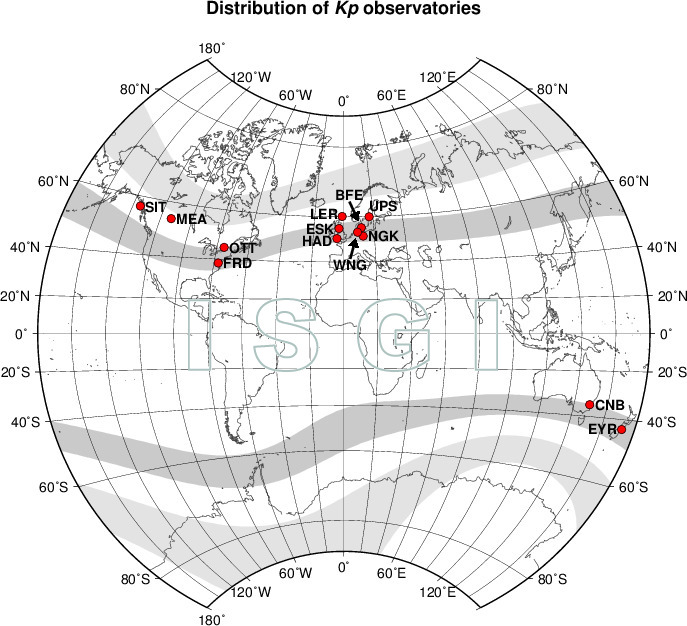
\includegraphics[width=\textwidth]{../figures_of_others/images/Kp_map.jpg}
		\captionoftiny{figure}{Courtesy of \href{http://isgi.unistra.fr/indices_kp.php}{International Service of Geomagnetic Indices (ISGI)}, 2013}
	\end{columns}
\end{frame}
\begin{frame}[c]{\Kp~index}{Quicklook \Kp{}}
	\begin{columns}[c]
	\column{0.5\textwidth}
		
		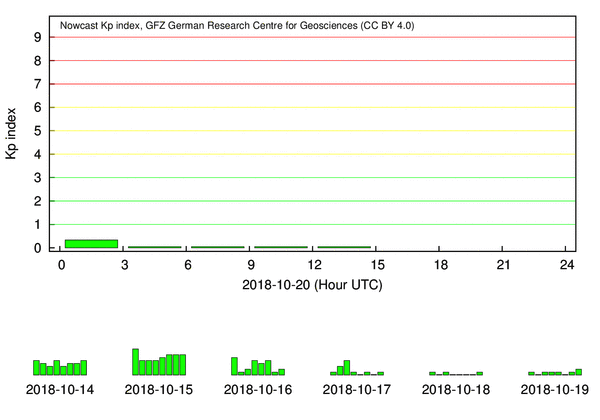
\includegraphics[width=\textwidth]{../talk_figures/ql_bar.png}
		\captionoftiny{figure}{Credit: \href{http://www.gfz-potsdam.de/en/kp-index/}{GFZ~Potsdam}, 2018}
	\end{columns}
\end{frame}

\begin{frame}[c]{Solar wind electric field}{}
	\begin{columns}[c]
	\column{0.5\textwidth}
		
% 		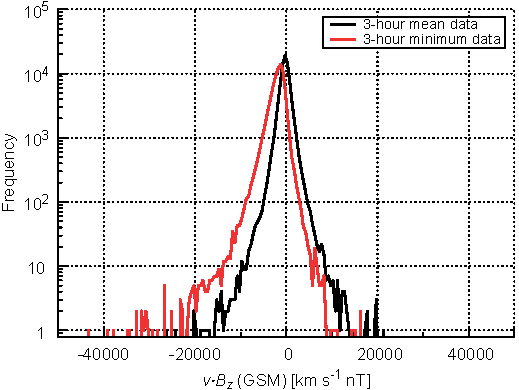
\includegraphics[width=\textwidth]{../figures_of_mine/chapter2/histogram_VBzgsm.pdf}
	% 	\captionoftiny{figure}{}

	\column{0.5\textwidth}

		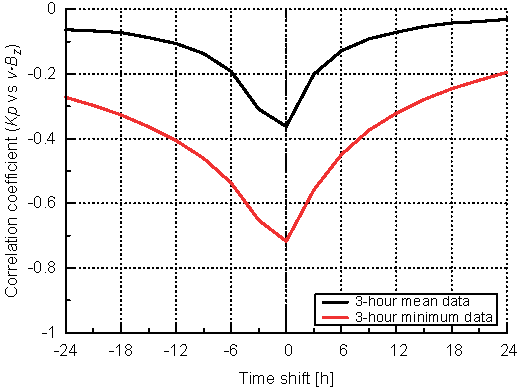
\includegraphics[width=\textwidth]{../figures_of_mine/chapter2/cc_lag_data_d_KpvsVBzgsm.pdf}
	% 	\captionoftiny{figure}{}
	
	\end{columns}
\end{frame}
\begin{frame}[c]{Solar wind electric field}{}
	\begin{columns}[c]
	\column{0.5\textwidth}
		
		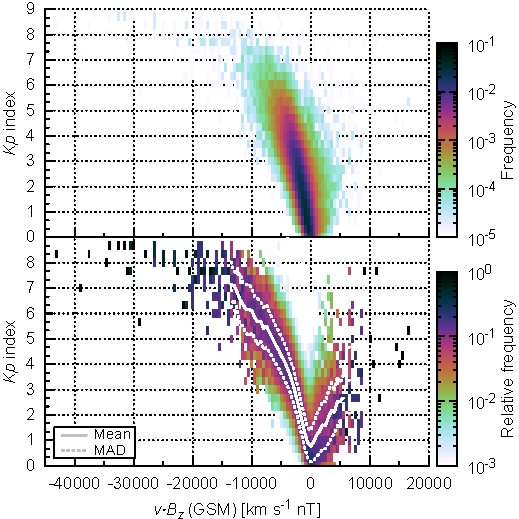
\includegraphics[width=\textwidth]{../figures_of_mine/chapter2/Kp_2dhistogram_VBzgsm_sws_e.pdf}
	% 	\captionoftiny{figure}{}

	\column{0.5\textwidth}

		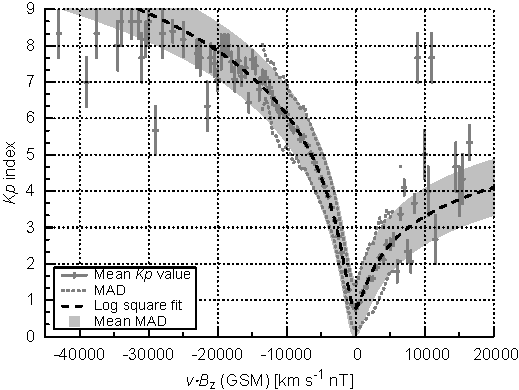
\includegraphics[width=\textwidth]{../figures_of_mine/chapter2/Kp_2dhistogram_VBzgsm_sws_fit_e.pdf}
	% 	\captionoftiny{figure}{}
	
	\end{columns}
\end{frame}
\begin{frame}[c]{Solar wind velocity}{}
	\begin{columns}[c]
	\column{0.5\textwidth}
		
% 		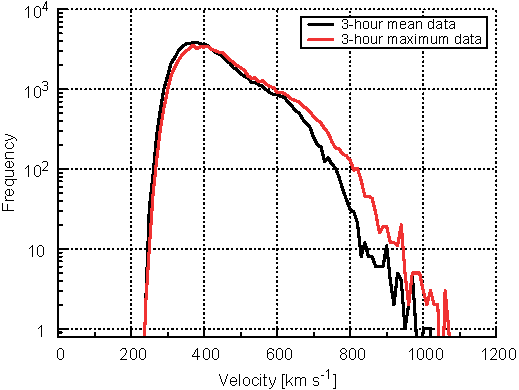
\includegraphics[width=\textwidth]{../figures_of_mine/chapter2/histogram_V_d.pdf}
	% 	\captionoftiny{figure}{}

	\column{0.5\textwidth}

		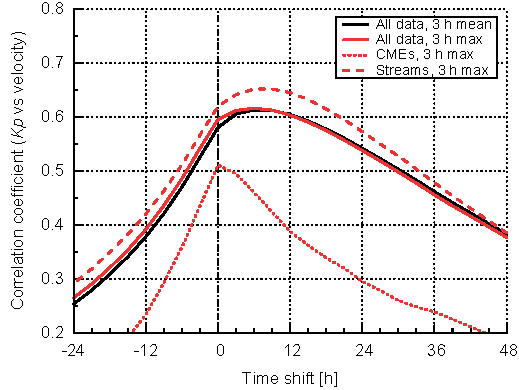
\includegraphics[width=\textwidth]{../figures_of_mine/chapter2/cc_lag_sws_f.pdf}
	% 	\captionoftiny{figure}{}
	
	\end{columns}
\end{frame}

\begin{frame}[c]{Solar wind velocity}{}
	CME -- stream separation
	
	Solar Wind Structures list
\end{frame}
\begin{frame}[c]{Solar wind velocity}{}
	\begin{columns}[c]
	\column{\textwidth}
		
		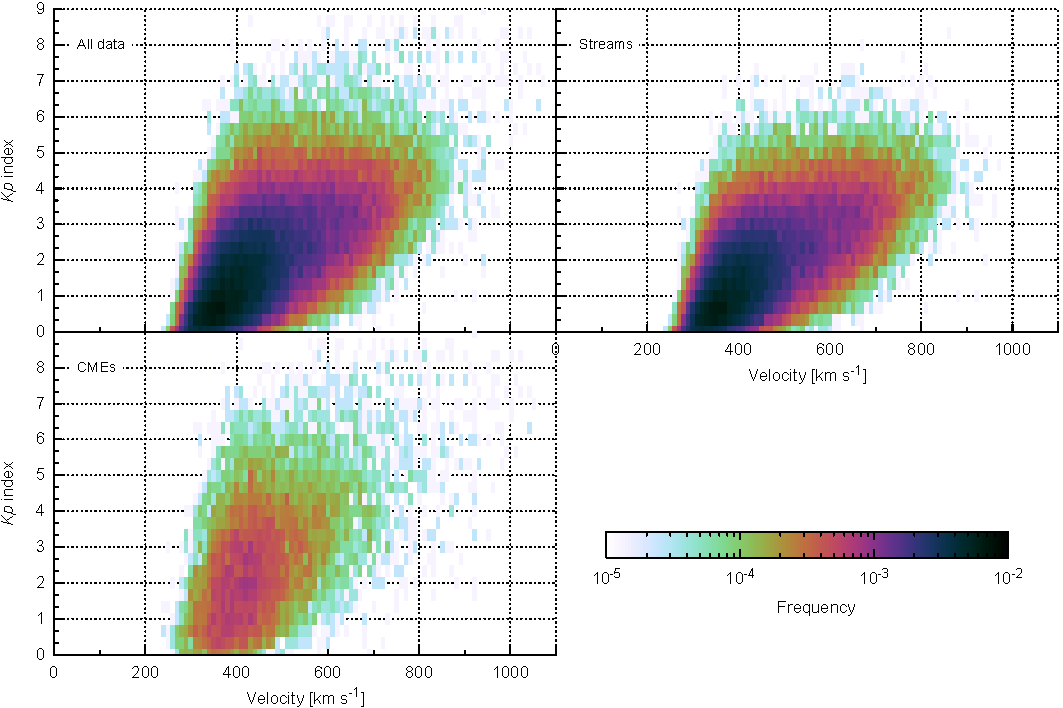
\includegraphics[width=0.8\textwidth]{../figures_of_mine/chapter2/Kp_2dhistogram_V_sws_e.pdf}
	% 	\captionoftiny{figure}{}

	\end{columns}
\end{frame}
\begin{frame}[c]{}{}
	\begin{columns}[c]
	\column{0.5\textwidth}
		
% 		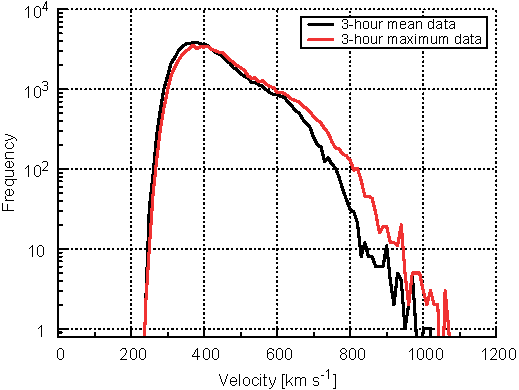
\includegraphics[width=\textwidth]{../figures_of_mine/chapter2/histogram_V_d.pdf}
	% 	\captionoftiny{figure}{}

	\column{0.5\textwidth}

		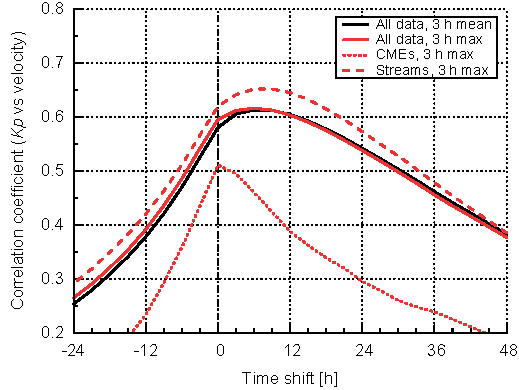
\includegraphics[width=\textwidth]{../figures_of_mine/chapter2/cc_lag_sws_f.pdf}
	% 	\captionoftiny{figure}{}
	
	\end{columns}
\end{frame}

\begin{frame}[c]{CME velocity}{}
	\begin{columns}[c]
	\column{0.5\textwidth}
		
		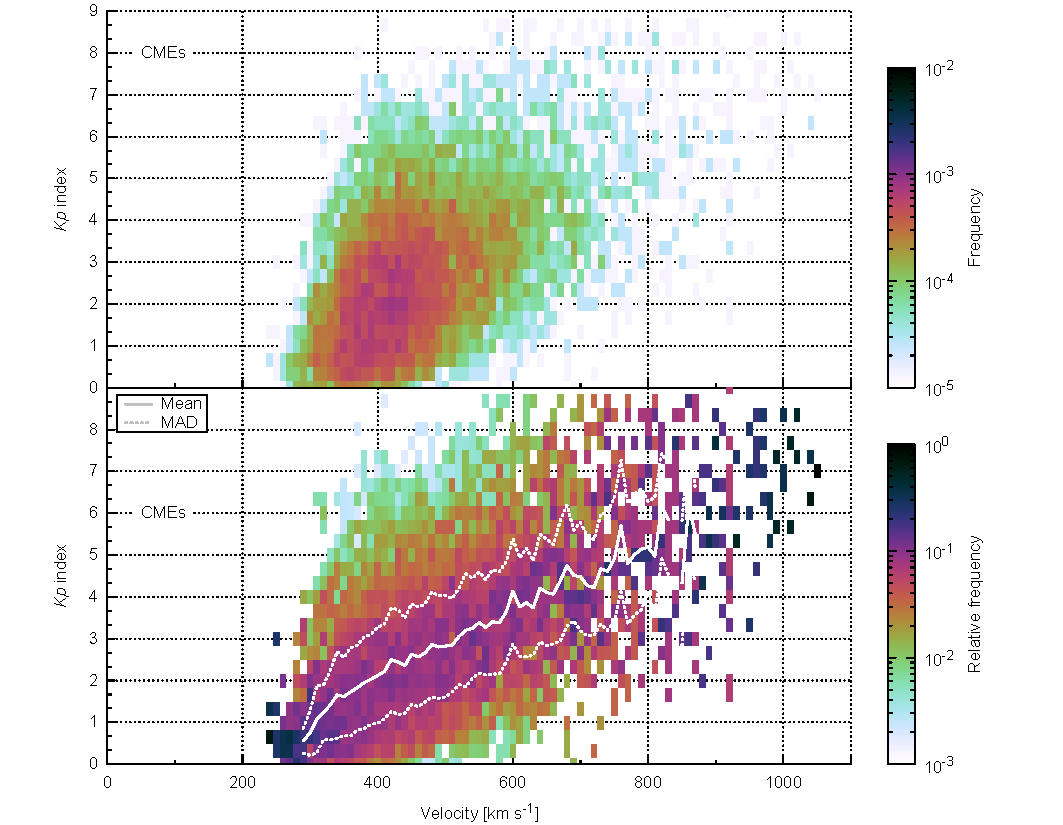
\includegraphics[width=\textwidth]{../figures_of_mine/chapter2/Kp_2dhistogram_V_sws1_d.pdf}
	% 	\captionoftiny{figure}{}

	\column{0.5\textwidth}

		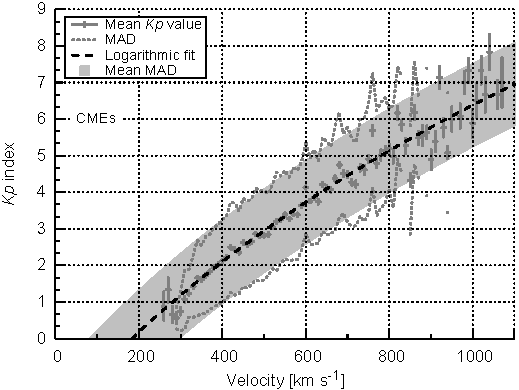
\includegraphics[width=\textwidth]{../figures_of_mine/chapter2/Kp_2dhistogram_V_sws1_fit_e.pdf}
	% 	\captionoftiny{figure}{}
	
	\end{columns}
\end{frame}
\begin{frame}[c]{Stream velocity}{}
	\begin{columns}[c]
	\column{0.5\textwidth}
		
		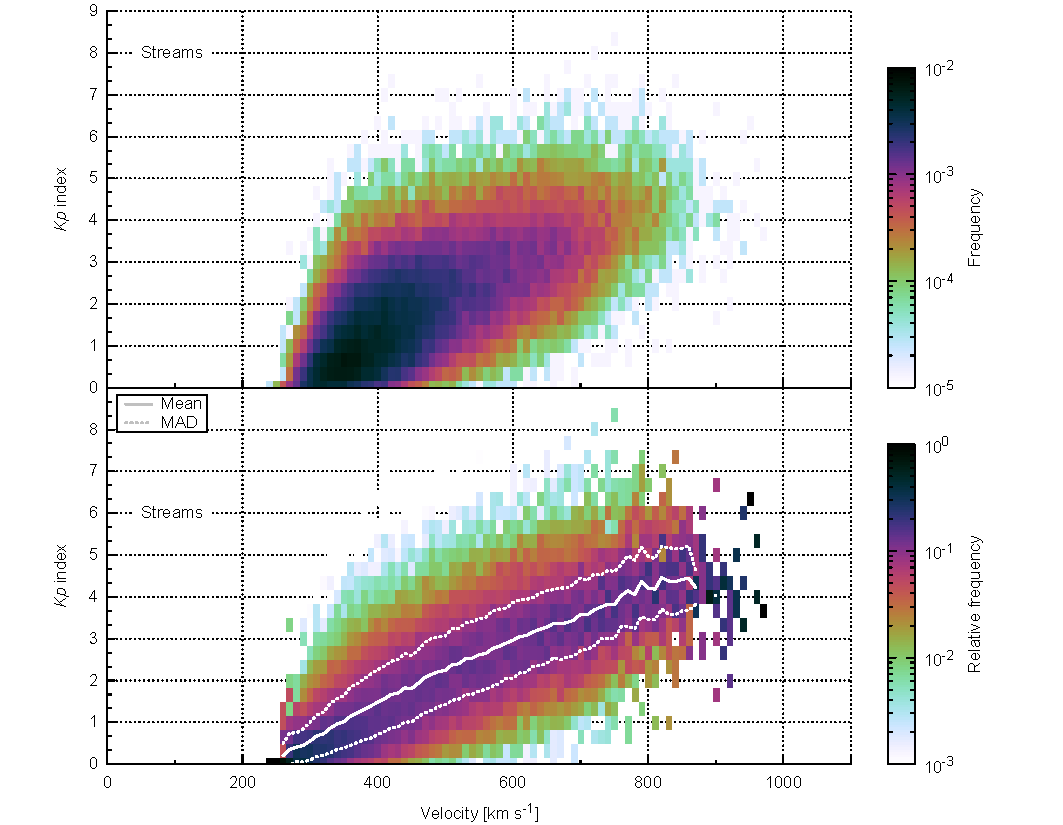
\includegraphics[width=\textwidth]{../figures_of_mine/chapter2/Kp_2dhistogram_V_sws23_e.pdf}
	% 	\captionoftiny{figure}{}

	\column{0.5\textwidth}

		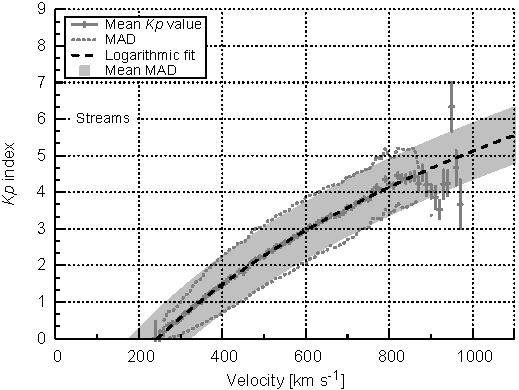
\includegraphics[width=\textwidth]{../figures_of_mine/chapter2/Kp_2dhistogram_V_sws23_fit_e.pdf}
	% 	\captionoftiny{figure}{}
	
	\end{columns}
\end{frame}
\begin{frame}[c]{}{}
	\begin{columns}[c]
	\column{\textwidth}
		
		\centering
		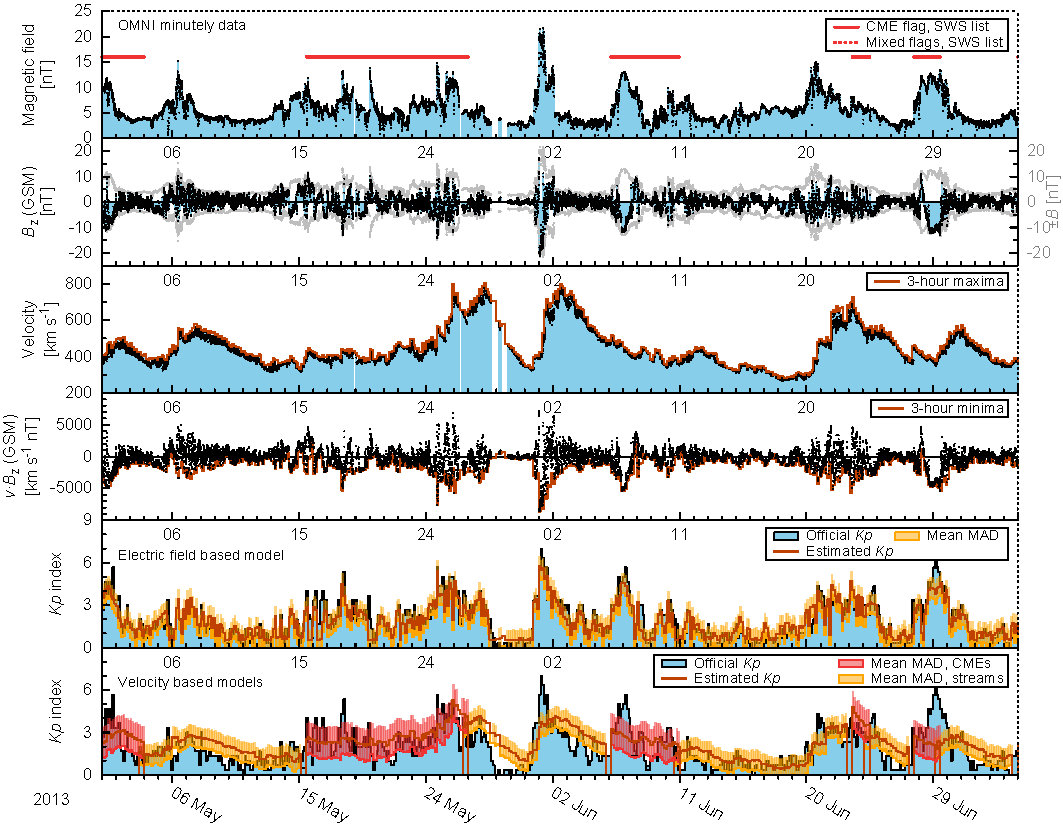
\includegraphics[width=0.8\textwidth]{../figures_of_mine/chapter2/example_sw_plot_1month_b_9hshift_2013-5-1_65.pdf}
	% 	\captionoftiny{figure}{}

	\end{columns}
\end{frame}
\begin{frame}[c]{}{}
	\begin{columns}[c]
	\column{\textwidth}
		\centering
		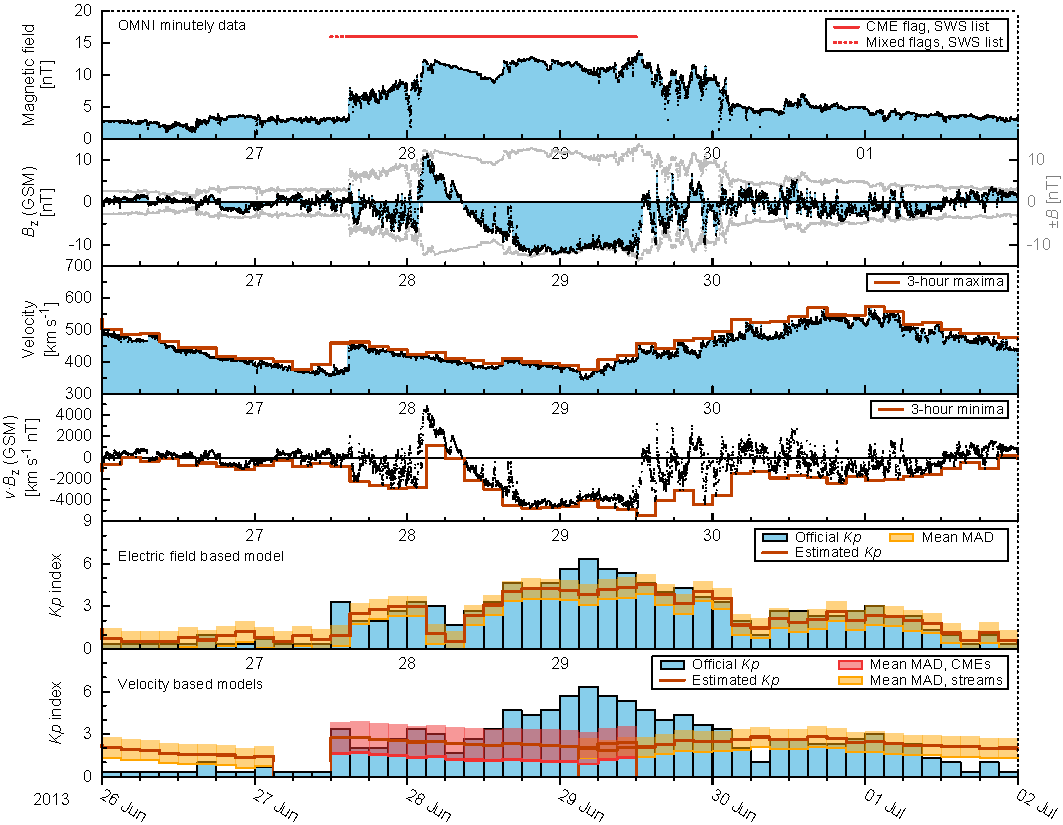
\includegraphics[width=0.8\textwidth]{../figures_of_mine/chapter2/example_sw_plot_CME_b_9hshift_2013-6-26_6.pdf}
	% 	\captionoftiny{figure}{}

	\end{columns}
\end{frame}
\begin{frame}[c]{}{}
	\begin{columns}[c]
	\column{0.5\textwidth}
		
		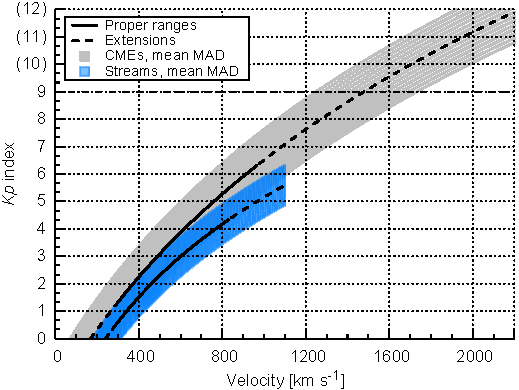
\includegraphics[width=\textwidth]{../figures_of_mine/chapter2/Kp_2dhistogram_V_sws123_fit_f3.pdf}
	% 	\captionoftiny{figure}{}

	\column{0.5\textwidth}

	\end{columns}
\end{frame}

\begin{frame}[c]{Results}{}
	\begin{columns}[c]
	\column{\textwidth}
		
		Predictive \Kp{} models based on relations with
		\begin{itemize}%[<+->]
			\item solar wind electric field proxy (\vBz{})
			\item velocity of CME-associated flows ($v_\text{CME}$)
			\item velocity of solar wind streams ($v_\text{stream}$)
		\end{itemize}
		
	\end{columns}
\end{frame}
\begin{frame}[c]{Conclusions}{}
% 	\begin{columns}[c]
% 	\column{\textwidth}
		
		\begin{itemize}%[<+->]
			\item The processing of 3-hour extrema of high time resolution data captures short-term geoeffective magnetic features that are neglected when averaging over 3-hour intervals
			\item The isolated treatment of CMEs and streams is beneficial to the prediction accuracy of \Kp{}
			\item The prediction models perform well for their limited input information
		\end{itemize}
		
% 	\end{columns}
	
	\vspace*{\fill} \hfill \hyperlink{prediction_performance}{\beamerskipbutton{Prediction performance}}
\end{frame}


\section{Solar wind model for the inner heliosphere}

\begin{frame}[c]{Sun--Earth evolution of the solar wind}{}
	Solar wind measured in-situ throughout the heliosphere -- except near-Sun
\end{frame}
\begin{frame}[c]{Sun--Earth evolution of the solar wind}{}
	special scientific interest:\\
	coronal heating\\
	solar wind acceleration
\end{frame}
\begin{frame}[c]{Sun--Earth evolution of the solar wind}{Aims}
	Solar wind model for the inner heliosphere and prediction of the near-Sun environment for the PSP orbit
\end{frame}

\begin{frame}[c]{Parker Solar Probe}{}
	\begin{columns}[c]
	\column{0.5\textwidth}
		
		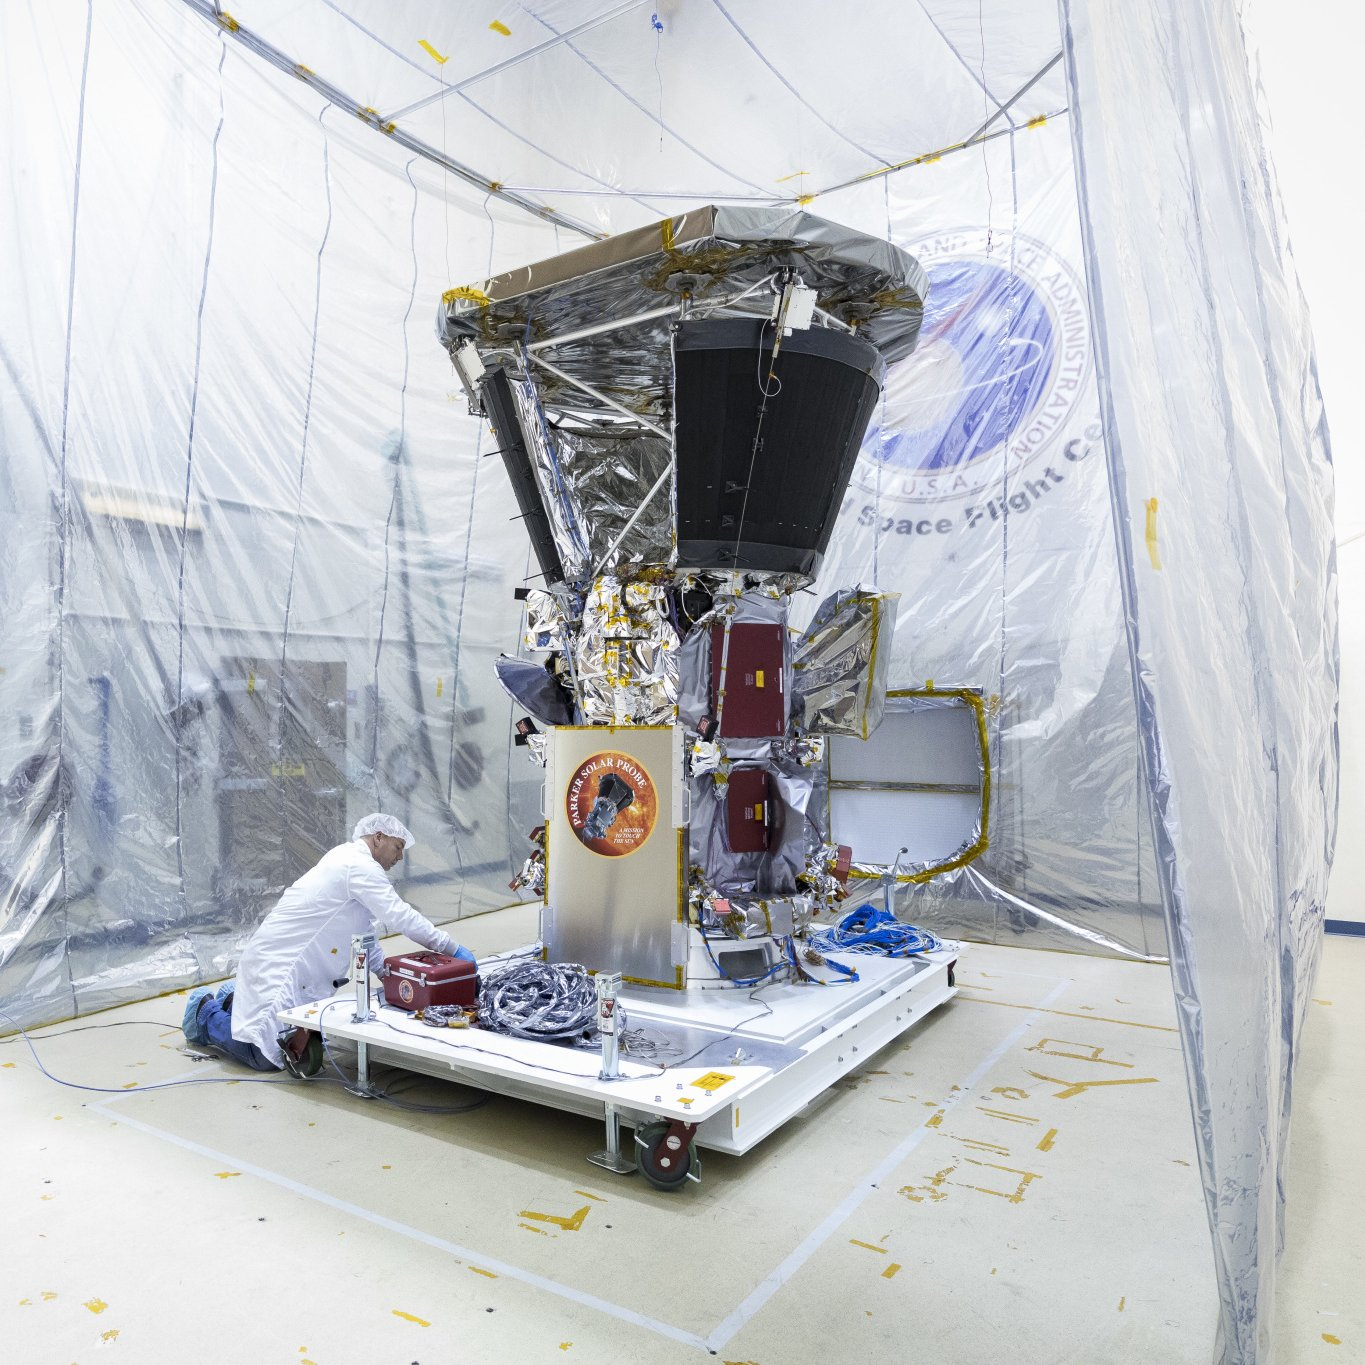
\includegraphics[width=\textwidth]{../figures_of_others/images/aa-roll-sc-into-acoustics-cell-0199_square.jpg}
		\captionoftiny{figure}{Credit: \href{http://parkersolarprobe.jhuapl.edu/News-Center/Show-Article.php?articleID=62}{NASA/Johns Hopkins APL/Ed Whitman}, 2017}

	\column<2>{0.5\textwidth}
		
		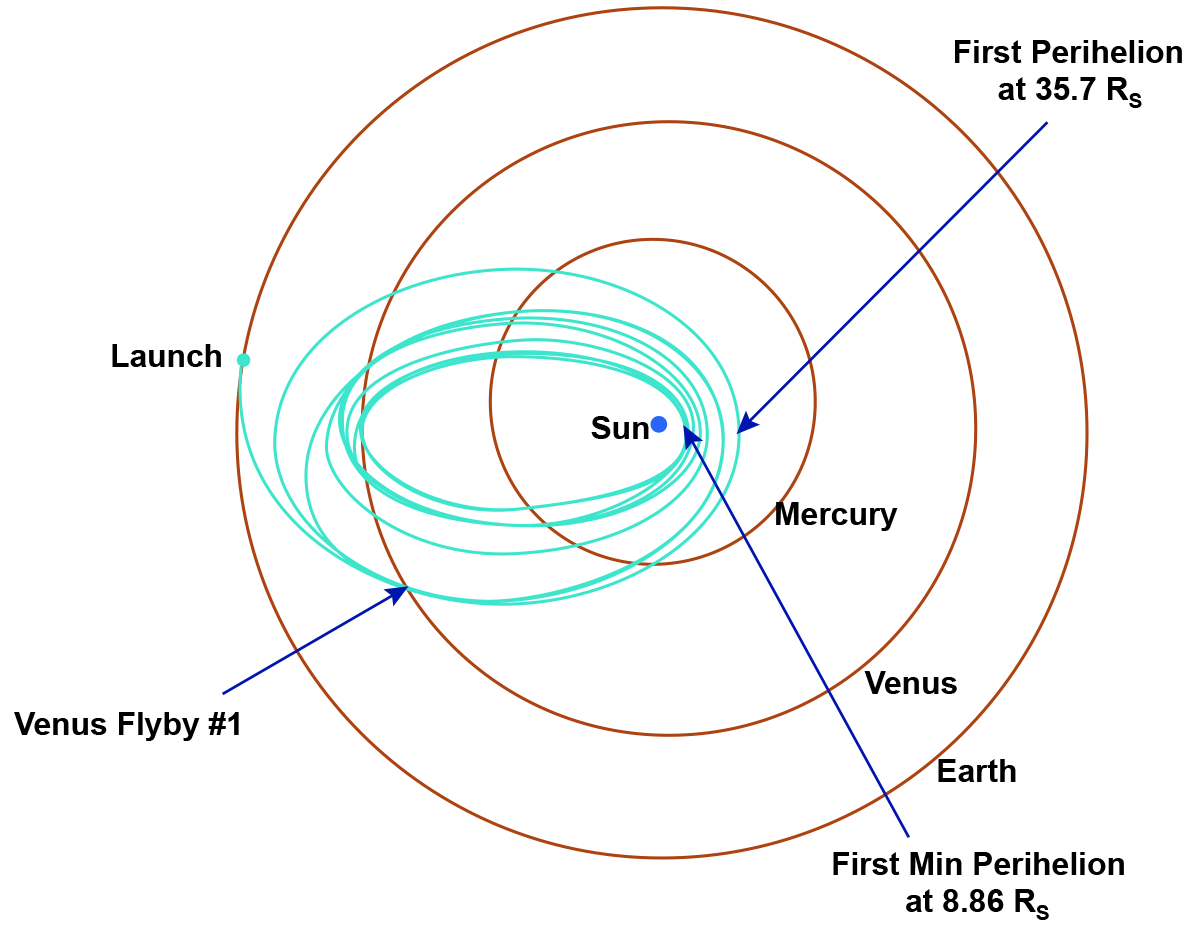
\includegraphics[width=\textwidth]{../figures_of_others/images/PSP_MissionDesign2_negative_crop.png}
		\captionoftiny{figure}{Credit: \href{http://parkersolarprobe.jhuapl.edu/The-Mission/index.php}{NASA/Johns Hopkins APL}, 2018}

	\end{columns}
\end{frame}
\begin{frame}[c]{Parker Solar Probe}{}
	\begin{columns}[c]
	\column{0.5\textwidth}
		
		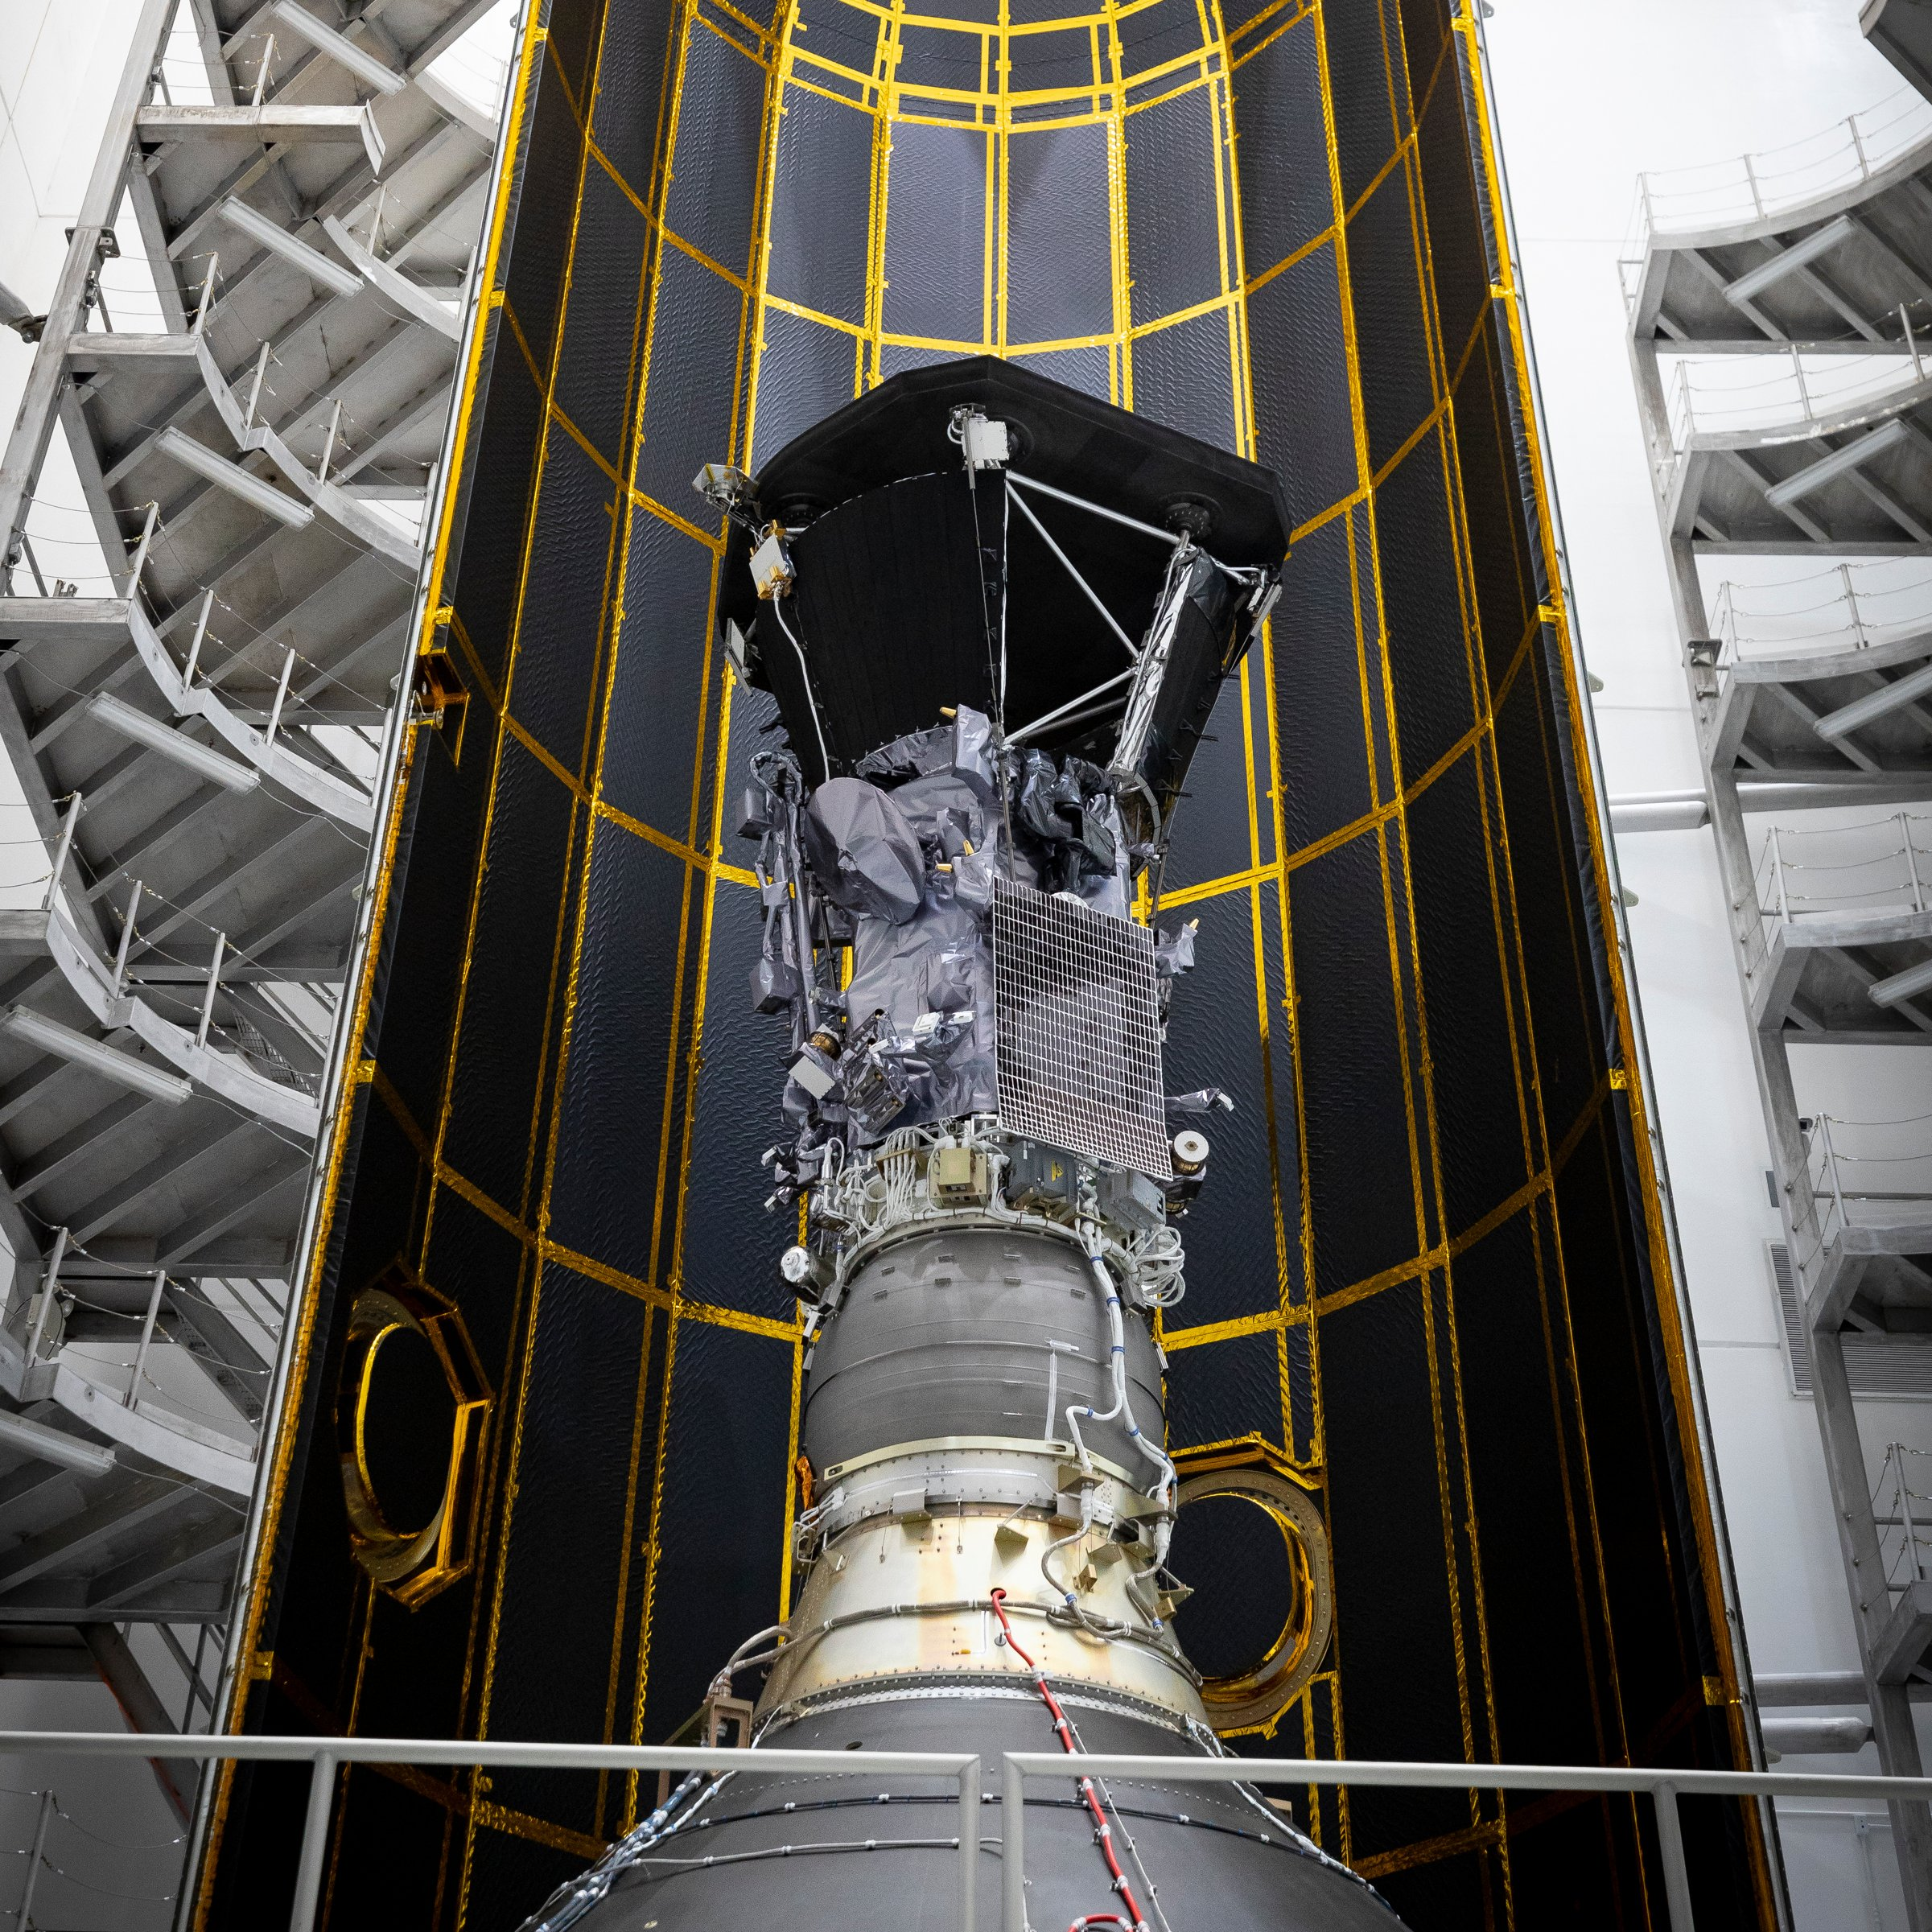
\includegraphics[width=\textwidth]{../figures_of_others/images/PSP_fencap2_square.jpg}
		\captionoftiny{figure}{Credit: \href{http://parkersolarprobe.jhuapl.edu/Multimedia/Images.php}{NASA/Johns Hopkins APL/Ed Whitman}, 2018}

	\column<2>{0.5\textwidth}

		launch date, Venus flyby, first perihelion
	\end{columns}
\end{frame}

\begin{frame}[c]{PSP's current position}{}
	\begin{columns}[t]	% [tcb] alignment relative to each column size
	\column{0.5\textwidth}
	
		\hspace*{-21pt}
		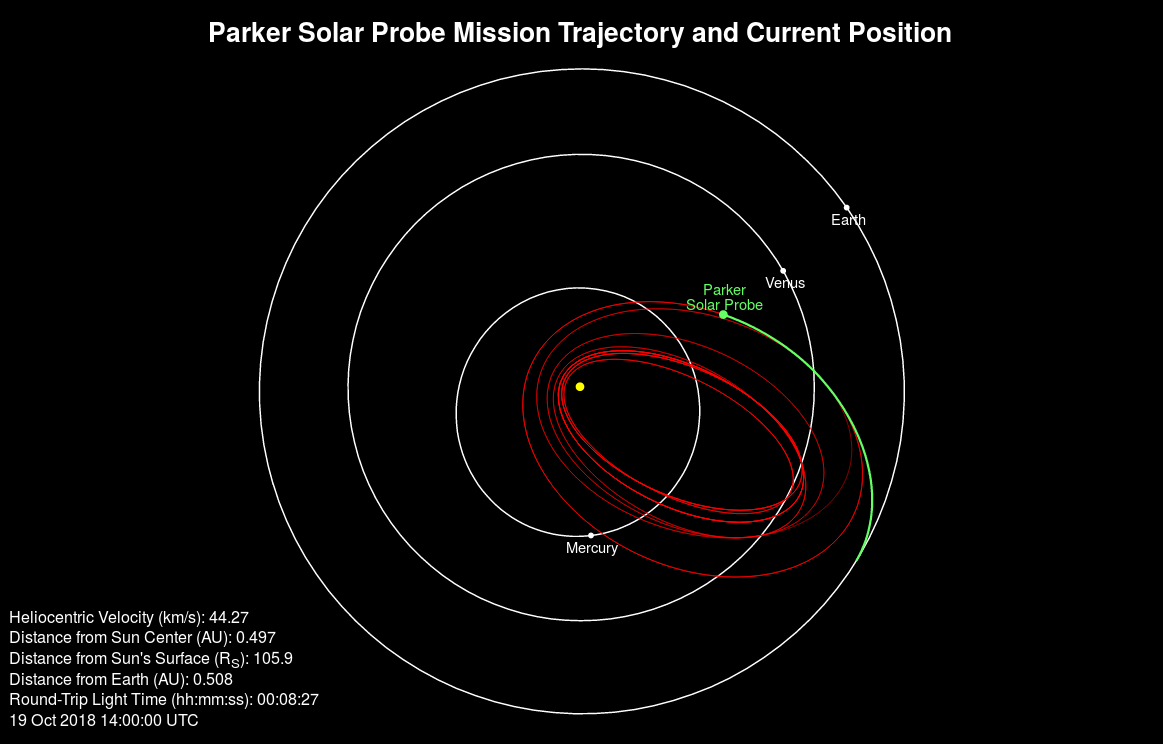
\includegraphics[height=0.85\textwidth]{../talk_figures/psp201810_0400_top.png}
		\captionoftiny{figure}{Credit: \href{http://parkersolarprobe.jhuapl.edu/The-Mission/index.php}{NASA}}

	\column{0.5\textwidth}
	
		\hspace*{-21pt}
		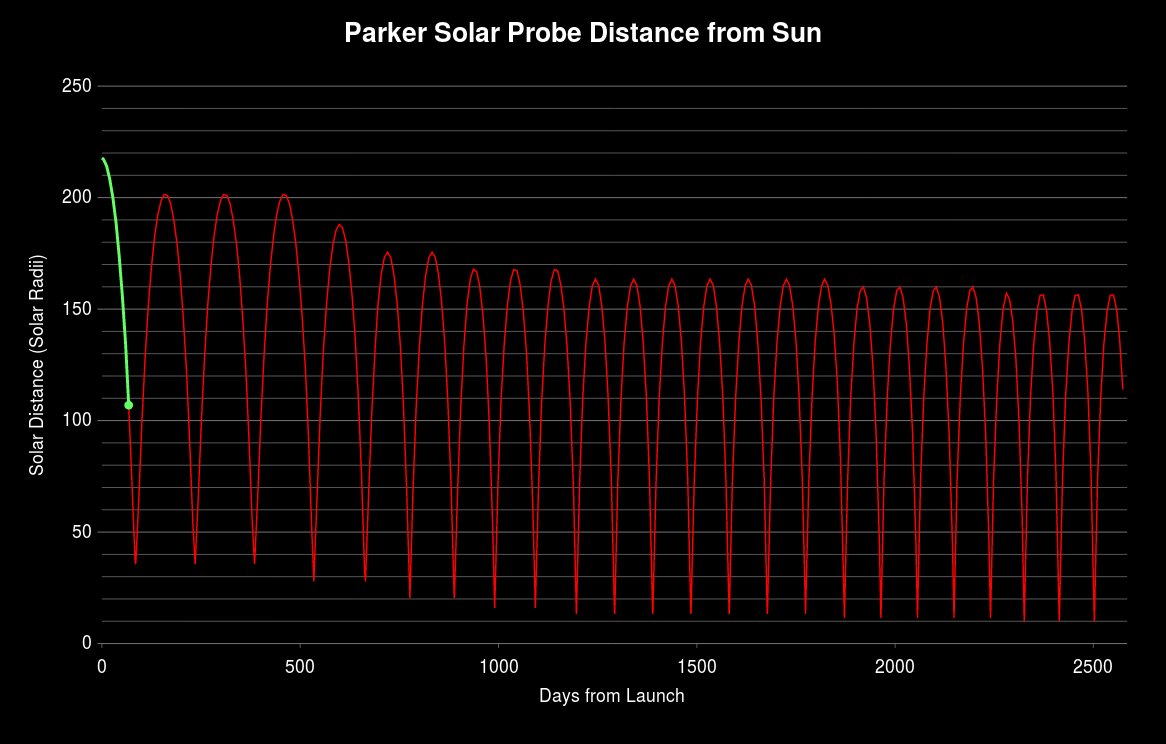
\includegraphics[height=0.85\textwidth]{../talk_figures/psp201810_0400_bottom.png}
% 		\captionoftiny{figure}{Credit: \href{http://parkersolarprobe.jhuapl.edu/The-Mission/index.php}{NASA}}
		
	\end{columns}
\end{frame}

\begin{frame}[c]{}{}
	motivation
\end{frame}
\begin{frame}[c]{Frequency distributions}{}
	\begin{columns}[c]	% [tcb] alignment relative to each column size
	\column{0.7\textwidth}
	
		\hspace*{-21pt}
		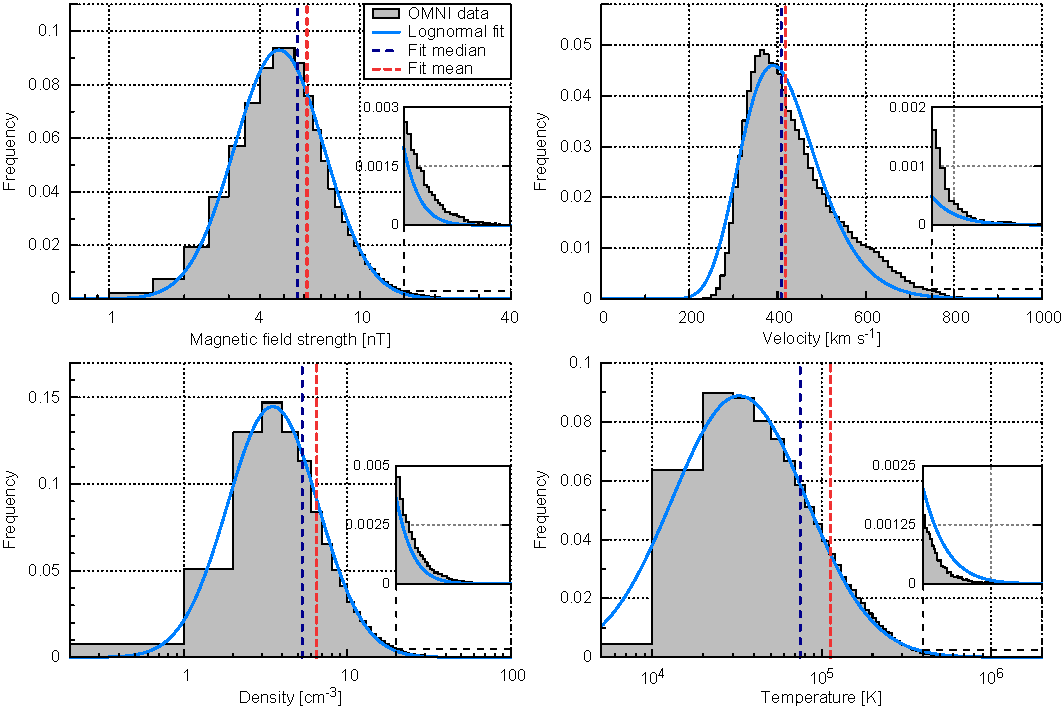
\includegraphics[width=1.1\textwidth]{../figures_paper/histogram_fits_4_a_zoom_paper_pdfplot.pdf}
	% 	\captionoftiny{figure}{}

	\column<2>{0.3\textwidth}
	
		\hspace*{-10pt}
		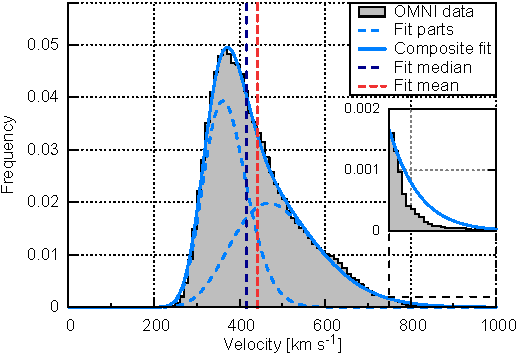
\includegraphics[width=1.2\textwidth]{../figures_paper/histogram_fits_V_a_zoom_dbl_paper_pdfplot.pdf}
	% 	\captionoftiny{figure}{}

	\end{columns}
	\vspace*{\fill} \hfill \hyperlink{lognormal_distribution}{\beamerskipbutton{Lognormal distribution}}
\end{frame}
\begin{frame}[c]{Sunspot number dependence}{}
	\begin{columns}[c]
	\column{0.5\textwidth}
		
		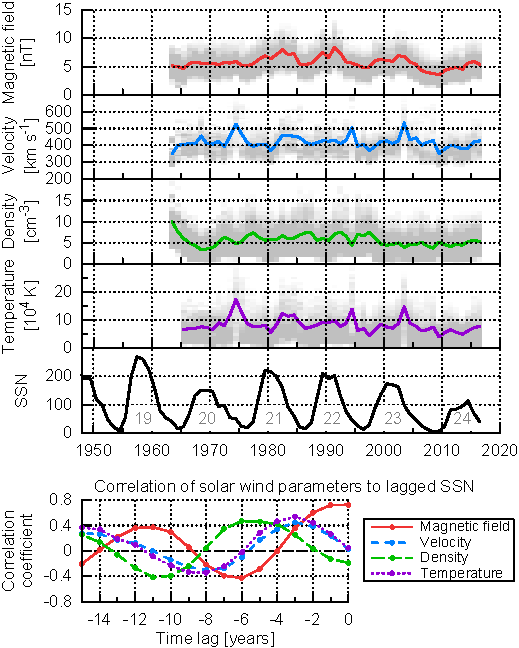
\includegraphics[width=\textwidth]{../figures_paper/OMNI_yearly_ssn_correlation_c_plot.pdf}
% 		\captionoftiny{figure}{}

	\column{0.5\textwidth}

	\end{columns}
\end{frame}
\begin{frame}[c]{Sunspot number dependence}{}
	\begin{columns}[c]
	\column{0.5\textwidth}
		
		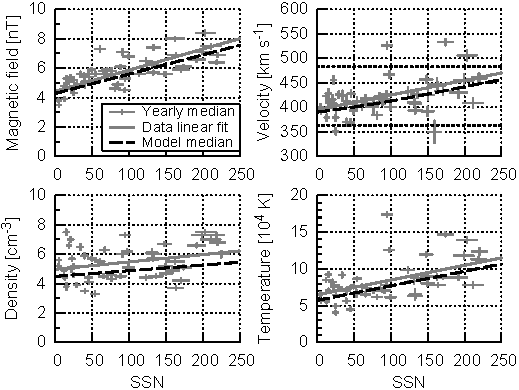
\includegraphics[width=\textwidth]{../figures_paper/OMNI_yearly_BVNTvsSSN_a.pdf}
% 		\captionoftiny{figure}{}

	\column{0.5\textwidth}

		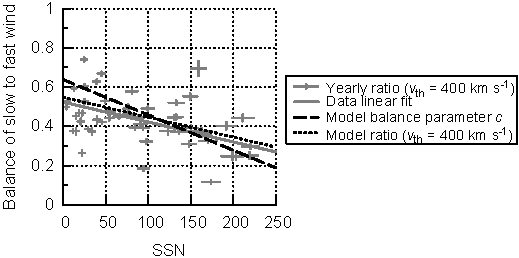
\includegraphics[width=\textwidth]{../figures_paper/Vdbl_SSN_ratio_f_plot.pdf}
% 		\captionoftiny{figure}{}

	\end{columns}
\end{frame}
\begin{frame}[c]{Sunspot number dependence}{}
	\centering
	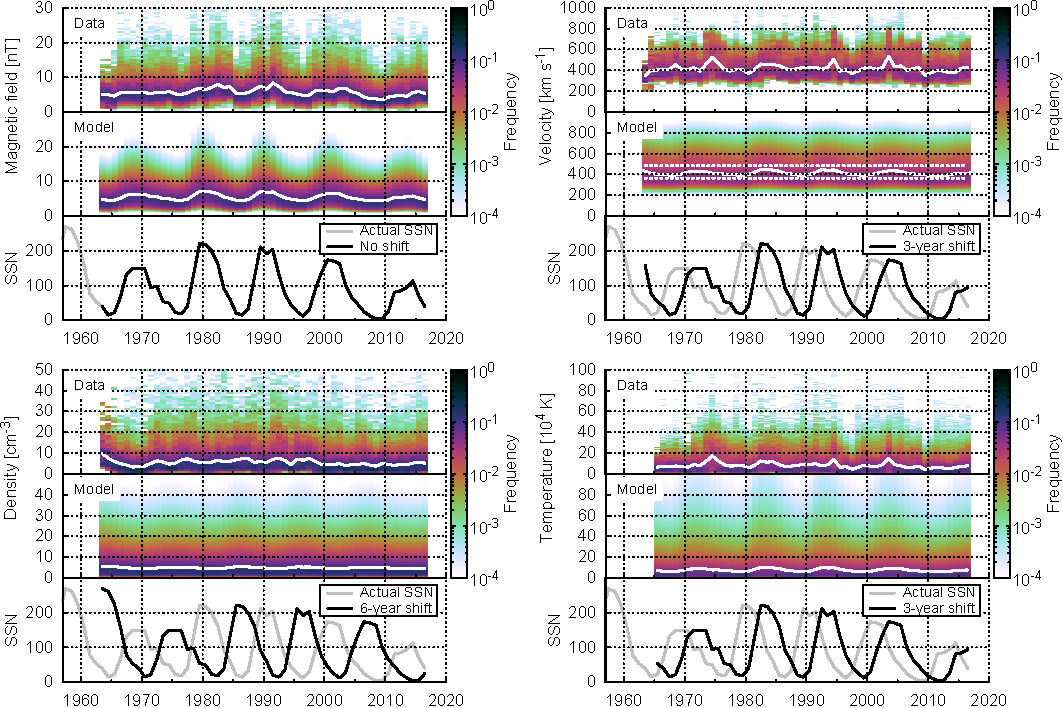
\includegraphics[width=0.8\textwidth]{../figures_paper/OMNI_yearly_BVdblNTSSN_fit_e_plot.pdf}
% 	\captionoftiny{figure}{}
\end{frame}

\begin{frame}[c]{Solar distance dependence}{}
	\centering
	\includegraphics[width=0.8\textwidth]{../figures_paper/mixed_fit_fixed_4_paper_f_plot.pdf}
% 	\captionoftiny{figure}{}
\end{frame}

\begin{frame}[c]{}{}
	combine models, extrapolation
\end{frame}
\begin{frame}[c]{SSN prediction}{}
	\begin{columns}[c]
	\column{0.5\textwidth}
		
		\includegraphics[width=\textwidth]{../figures_paper/SPP_orbit_predicted_SSN_overview_f_plot.pdf}
% 		\captionoftiny{figure}{}

	\column{0.5\textwidth}

	\end{columns}
\end{frame}

\begin{frame}[c]{PSP orbit prediction}{}
	\begin{columns}[c]
	\column{0.5\textwidth}
		
		\centering
		First perihelion (9.86~\Rs)\\\ 
		
		\includegraphics[width=\textwidth]{../figures_paper/SPP_perihelia_prediction_f_plot.pdf}

	\column<2>{0.5\textwidth}
	
		\centering
		First closest perihelion (36.7~\Rs)\\\ 
		
		\includegraphics[width=\textwidth]{../figures_paper/SPP_perihelia_prediction_nearest_f_plot.pdf}

	\end{columns}
\end{frame}
\begin{frame}[c]{PSP perihelia prediction}{}
	\begin{columns}[c]
	\column{0.6\textwidth}
		
		\includegraphics[width=\textwidth]{../figures_paper/SPP_sw_distributions_b.pdf}

	\column{0.4\textwidth}

	\end{columns}
\end{frame}

\begin{frame}[c]{Results}{}
	\begin{columns}[c]
	\column{\textwidth}
		
		\begin{itemize}%[<+->]
			\item Empirical solar wind model for the inner heliosphere
			\item Solar wind predictions for the PSP orbit
		\end{itemize}
		
	\end{columns}
\end{frame}
\begin{frame}[c]{Conclusions}{}
	\begin{columns}[c]
	\column{\textwidth}
		
		\begin{itemize}%[<+->]
			\item Velocity discrepancy -> Solar wind is still being accelerated up to 20\,\Rs{}
			\item Temperature discrepancy -> Solar wind is still being heated up to 20\,\Rs{}
		\end{itemize}
		
	\end{columns}
\end{frame}


\section{End matter}

\begin{frame}[c]{Thank you!}{}
	\begin{columns}[c]
	\column{0.5\textwidth}
		
	\column{0.5\textwidth}

	\end{columns}
\end{frame}


\begin{frame}[t,allowframebreaks]{References}
	\tiny
	\begin{thebibliography}{10}
	
		\beamertemplatebookbibitems
		
		\beamertemplatearticlebibitems
		
		
\bibitem[{{Bothmer} \& {Schwenn}(1998)}]{Bothmer1998}
	{Bothmer}, V. \& {Schwenn}, R. 1998, \emph{{The structure and origin of magnetic clouds in the solar
	wind}}, Annales Geophysicae, 16, 1,
	\href{http://dx.doi.org/10.1007/s00585-997-0001-x}{[DOI]},
	\href{http://adsabs.harvard.edu/abs/1998AnGeo..16....1B}{[ADS]}.

\bibitem[{{Cranmer} \& {van Ballegooijen}(2005)}]{Cranmer2005}
	{Cranmer}, S.~R. \& {van Ballegooijen}, A.~A. 2005, \emph{{On the Generation,
	Propagation, and Reflection of Alfv{\'e}n Waves from the Solar Photosphere to
	the Distant Heliosphere}}, \apjs, 156, 265,
	\href{http://dx.doi.org/10.1086/426507}{[DOI]},
	\href{http://adsabs.harvard.edu/abs/2005ApJS..156..265C}{[ADS]}.

\bibitem[{Davies(1990)}]{Davies1990}
	Davies, K. 1990, \emph{Ionospheric Radio} (Institution of Engineering and
	Technology),
	\href{http://digital-library.theiet.org/content/books/ew/pbew031e}{[link]},
	\href{http://dx.doi.org/10.1049/PBEW031E}{[DOI]}.

\bibitem[{{Hathaway}(2015)}]{Hathaway2015}
	{Hathaway}, D.~H. 2015, \emph{{The Solar Cycle}}, Living Reviews in Solar
	Physics, 12, 4, \href{http://dx.doi.org/10.1007/lrsp-2015-4}{[DOI]},
	\href{http://adsabs.harvard.edu/abs/2015LRSP...12....4H}{[ADS]}.

\bibitem[{{Hughes}(1995)}]{Hughes1995}
	{Hughes}, W.~J. 1995, \emph{{Chapter 9: The magnetopause, magnetotail, and
	magnetic reconnection}}, ed. M.~Kivelson \& C.~Russell, Introduction to Space
	Physics (Cambridge University Press, Cambridge), 227--287,
	\href{http://adsabs.harvard.edu/abs/1995isp..book.....K}{[ADS]}.

\bibitem[{{Marubashi} \& {Lepping}(2007)}]{Marubashi2007}
	{Marubashi}, K. \& {Lepping}, R.~P. 2007, \emph{{Long-duration magnetic clouds:
	a comparison of analyses using torus- and cylinder-shaped flux rope models}},
	Annales Geophysicae, 25, 2453,
	\href{http://dx.doi.org/10.5194/angeo-25-2453-2007}{[DOI]},
	\href{http://adsabs.harvard.edu/abs/2007AnGeo..25.2453M}{[ADS]}.
	
\bibitem[{{McComas} {et~al.}(2008{\natexlab{a}}){McComas}, {Ebert}, {Elliott},
	{Goldstein}, {Gosling}, {Schwadron}, \& {Skoug}}]{McComas200809}
	{McComas}, D.~J., {Ebert}, R.~W., {Elliott}, H.~A. {et~al.} 2008{\natexlab{a}},
	\emph{{Weaker solar wind from the polar coronal holes and the whole Sun}},
	\grl, 35, L18103, \href{http://dx.doi.org/10.1029/2008GL034896}{[DOI]},
	\href{http://adsabs.harvard.edu/abs/2008GeoRL..3518103M}{[ADS]}.

\bibitem[{{Owens} \& {Forsyth}(2013)}]{Owens2013}
	{Owens}, M.~J. \& {Forsyth}, R.~J. 2013, \emph{{The Heliospheric Magnetic
	Field}}, Living Reviews in Solar Physics, 10, 5,
	\href{http://dx.doi.org/10.12942/lrsp-2013-5}{[DOI]},
	\href{http://adsabs.harvard.edu/abs/2013LRSP...10....5O}{[ADS]}.

\bibitem[{{Parker}(1958)}]{Parker1958}
	{Parker}, E.~N. 1958, \emph{{Dynamics of the Interplanetary Gas and Magnetic Fields.}}, \apj, 128, 664, \href{http://dx.doi.org/10.1086/146579}{[DOI]}, \href{http://adsabs.harvard.edu/abs/1958ApJ...128..664P}{[ADS]}.

\bibitem[{{Pizzo}(1991)}]{Pizzo1991}
	{Pizzo}, V.~J. 1991, \emph{{The evolution of corotating stream fronts near the
	ecliptic plane in the inner solar system. II - Three-dimensional
	tilted-dipole fronts}}, \jgr, 96, 5405,
	\href{http://dx.doi.org/10.1029/91JA00155}{[DOI]},
	\href{http://adsabs.harvard.edu/abs/1991JGR....96.5405P}{[ADS]}.
	
\bibitem[{{Schatten} {et~al.}(1969){Schatten}, {Wilcox}, \&
	{Ness}}]{Schatten1969}
	{Schatten}, K.~H., {Wilcox}, J.~M. \& {Ness}, N.~F. 1969, \emph{{A model of
	interplanetary and coronal magnetic fields}}, \solphys, 6, 442,
	\href{http://dx.doi.org/10.1007/BF00146478}{[DOI]},
	\href{http://adsabs.harvard.edu/abs/1969SoPh....6..442S}{[ADS]}.

\bibitem[{{Venzmer} \& {Bothmer}(2018)}]{Venzmer2018}
	{Venzmer}, M.~S. \& {Bothmer}, V. 2018, \emph{{Solar-wind predictions for the
	Parker Solar Probe orbit. Near-Sun extrapolations derived from an empirical
	solar-wind model based on Helios and OMNI observations}}, \aap, 611, A36,
	\href{http://dx.doi.org/10.1051/0004-6361/201731831}{[DOI]},
	\href{http://adsabs.harvard.edu/abs/2018A\%26A...611A..36V}{[ADS]}.



	\end{thebibliography}
\end{frame}


\appendix

\section{Backup slides}

\subsection{Solar wind}

\begin{frame}[c,label=butterfly]{Solar activity}{Magnetic butterfly diagram}
% 	\hypertarget{butterfly}{\beamerbutton{I'm on this slide}}
	
	\centering
	\includegraphics[width=0.9\textwidth]{../figures_of_others/images/Hathaway_magbfly_201804_cropped.png}
	\captionoftiny{figure}{\centering Courtesy of David~Hathaway, \href{http://solarcyclescience.com/solarcycle.html}{Solar Cycle Science}, 2018, updated version of {\citet[Fig.~17]{Hathaway2015}}}
\end{frame}

\subsection{Chapter2}

\begin{frame}[c]{\Kp{} long-term variations}{}
	\begin{columns}[c]
	\column{0.5\textwidth}
		
		\includegraphics[width=\textwidth]{../figures_of_mine/chapter2/Kp_histogram_yearlySSN_b.pdf}
% 		\captionoftiny{figure}{}
		
	\column{0.5\textwidth}
		
		\includegraphics[width=\textwidth]{../figures_of_mine/chapter2/Kp_histogram_monthly.pdf}
% 		\captionoftiny{figure}{}
	\end{columns}
\end{frame}

\begin{frame}[c,label=prediction_performance]{Prediction performance}{}
	\begin{columns}[c]
	\column{0.5\textwidth}
		
		\includegraphics[width=\textwidth]{../figures_of_mine/chapter2/model_performance_d.pdf}
	% 	\captionoftiny{figure}{}

	\column{0.5\textwidth}

		\includegraphics[width=\textwidth]{../figures_of_mine/chapter2/true_skill_score.pdf}
	% 	\captionoftiny{figure}{}
	
	\end{columns}
\end{frame}

\subsection{SW model}

\begin{frame}[c,label=lognormal_distribution]{Lognormal distribution}{}
	\begin{columns}[c]
	\column{0.5\textwidth}
		
	\includegraphics[width=\textwidth]{../figures_of_mine/gnuplots/lognormal_semi_log.pdf}
% 	\captionoftiny{figure}{}

	\column{0.5\textwidth}
	
	Probability density function:
	\begin{align}
		f(x) &= \frac{1}{\sigma \sqrt{2 \pi} x} \, \text{e}^{- \frac{(\ln x - \mu)^2}{2 \sigma^2}}	\nonumber
	\end{align}
	Location ($\mu$) and shape parameter ($\sigma$)
	
	\end{columns}
\end{frame}

% 
\section{Test slides}

\begin{frame}[c]{first slide}{A bit more information about this}
	This is a text in first frame. \pause This is a text in first frame. This is a text in first frame.
	\begin{definition}
		A definition
	\end{definition}
	\url{https://www.sharelatex.com/learn/latex/Beamer}
\end{frame}

\begin{frame}[<+->]{Ein Demotitel}{}
	\begin{itemize}
		\item<1-> dasgfs
		\item<2> asgag
		\item<3-> asgag
		\item asgag
	\end{itemize}
\end{frame}

\begin{frame}[<+->]{Ein Demotitel}{}
	\begin{itemize}
		\item dasgfs
		\item asgag
		\item asgag
		\item<.-> asgag
	\end{itemize}
\end{frame}

\begin{frame}{Ein Demotitel}{}
	\begin{itemize}
		\item<+-> dasgfs
		\item<+-> asgag
		\item<+-> asgag
		\item<+-> asgag
	\end{itemize}
\end{frame}
\begin{frame}{Ein Demotitel}{}
	\begin{itemize}[<+->]
		\item dasgfs
		\item asgag
		\item asgag
		\item asgag
	\end{itemize}
\end{frame}

\section{part two}

\begin{frame}[t]{Sample frame title}{}
	
	In this slide, some important text will be
	\alert<2->{highlighted} beause it's important.
	Please, don't abuse it.
	
	\onslide<2>{	%\uncover{}
	\begin{block}{Remark}
	Sample text
	\end{block}
	}
	
	\onslide*<1>{	%\only{}
	\begin{examples}
	Sample text in green box. "Examples" is fixed as block title.
	\end{examples}
	}
	
	\onslide+<2>{	%\visible{}
	\begin{alertblock}{Important theorem}
	Sample text in red box
	\end{alertblock}
	}
	
\end{frame}

\begin{frame}[plain]{Sample frame title}{}
	
	In this slide, some important text will be
	\alert{highlighted} beause it's important.
	Please, don't abuse it.
	
	\begin{block}{Remark}
	Sample text
	\end{block}
	
	\begin{alertblock}{Important theorem}
	Sample text in red box
	\end{alertblock}
	
	\begin{examples}
	Sample text in green box. "Examples" is fixed as block title.
	\end{examples}
\end{frame}

\section{part 3}

\begin{frame}{Two-column slide}{}
	\begin{columns}[t]
		\column{0.5\textwidth}
		This is a text in first column.
		$$E=mc^2$$
		\begin{itemize}
		\item First item
		\item Second item
		\end{itemize}
		
		\column{0.5\textwidth}
		This text will be in the second column
		and on a second tought this is a nice looking
		layout in some cases \citep{Venzmer2018}.
	\end{columns}
\end{frame}

\begin{frame}[t]{Sample}{}
	
	In this slide, some important text will be
	\alert<2->{highlighted} beause it's important.
	Please, don't abuse it.
	
	\begin{block}<1->{Remark}
	Sample text
	\end{block}
	
	\begin{examples}<2>
	Sample text in green box. "Examples" is fixed as block title.
	\end{examples}
	
	\begin{alertblock}<3>{Important theorem}
	Sample text in red box
	\end{alertblock}
	
\end{frame}

\section{Backup slides 2}

\begin{frame}{backup slide}{}
	gj
	
	\hyperlink{butterfly}{\beamerbutton{Magnetic butterfly diagram}}
	
	\hyperlink{butterfly}{\beamergotobutton{Go to my frame}}
	
	\hyperlink{butterfly}{\beamerreturnbutton{Back}}
	
	\hyperlink{butterfly}{\beamerskipbutton{butterfly page}}
\end{frame}

% \begin{frame}[]{title}{subtitle}
%
% \end{frame}
 



\end{document}


